\documentclass{article}
\usepackage{graphicx} % Required for inserting images
\usepackage{rotating}

%\renewcommand{\thepage}{S\arabic{page}}
\renewcommand{\thesection}{S\arabic{section}}
\renewcommand{\thetable}{S\arabic{table}}
\renewcommand{\thefigure}{S\arabic{figure}}

\title{Supplementary Data for: Urban Ozone Trends in Europe and the USA (2000-2021)}
\date{}
\begin{document}

\maketitle
\clearpage


%%%%%% regression bars %%%%%%

\begin{figure}[p]
\centering
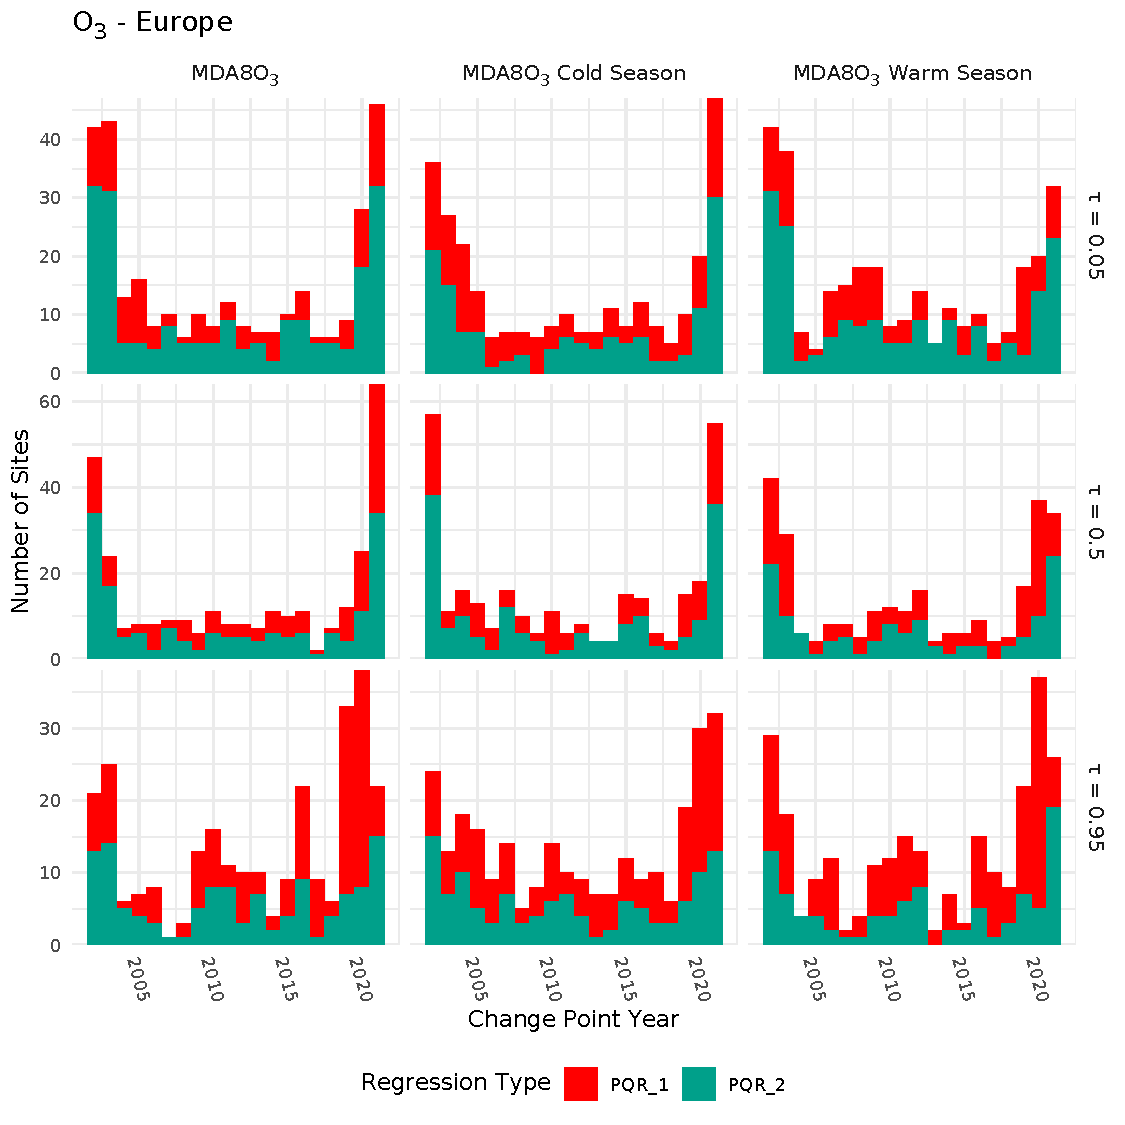
\includegraphics[width=\linewidth]{figures/si_figures/fS01_cp_year_o3_Europe.pdf}
\caption{Stacked bars showing years where change points have been assigned in }
\label{si_fig:cp_year_eu}
\end{figure}
\clearpage

\begin{figure}[p]
\centering
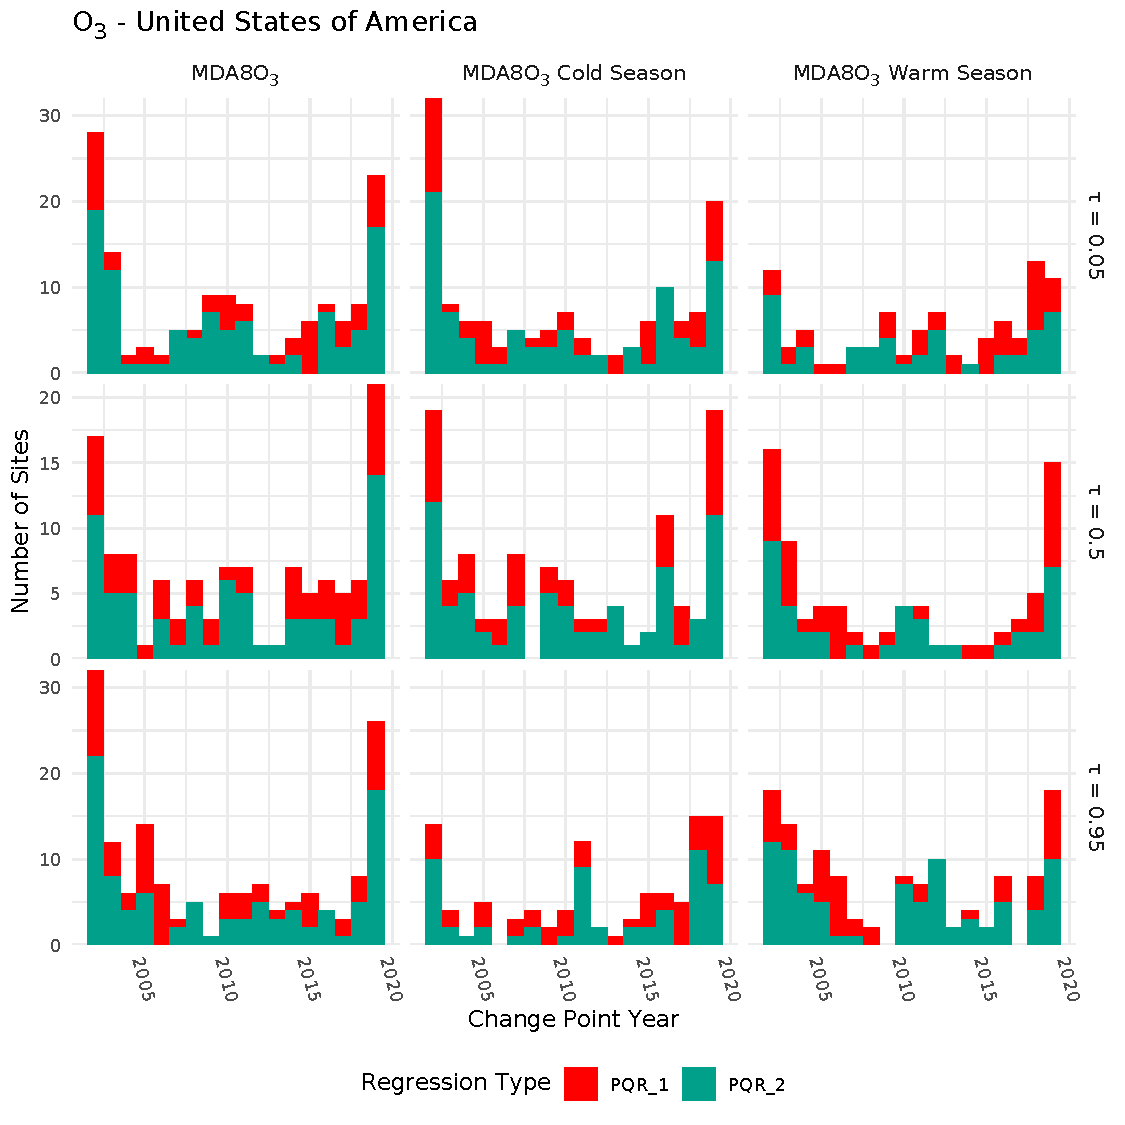
\includegraphics[width=\linewidth]{figures/si_figures/fS02_cp_year_o3_United-States-of-America.pdf}
\caption{}
\label{si_fig:cp_year_usa}
\end{figure}
\clearpage

\begin{sidewaysfigure}[p]
\centering
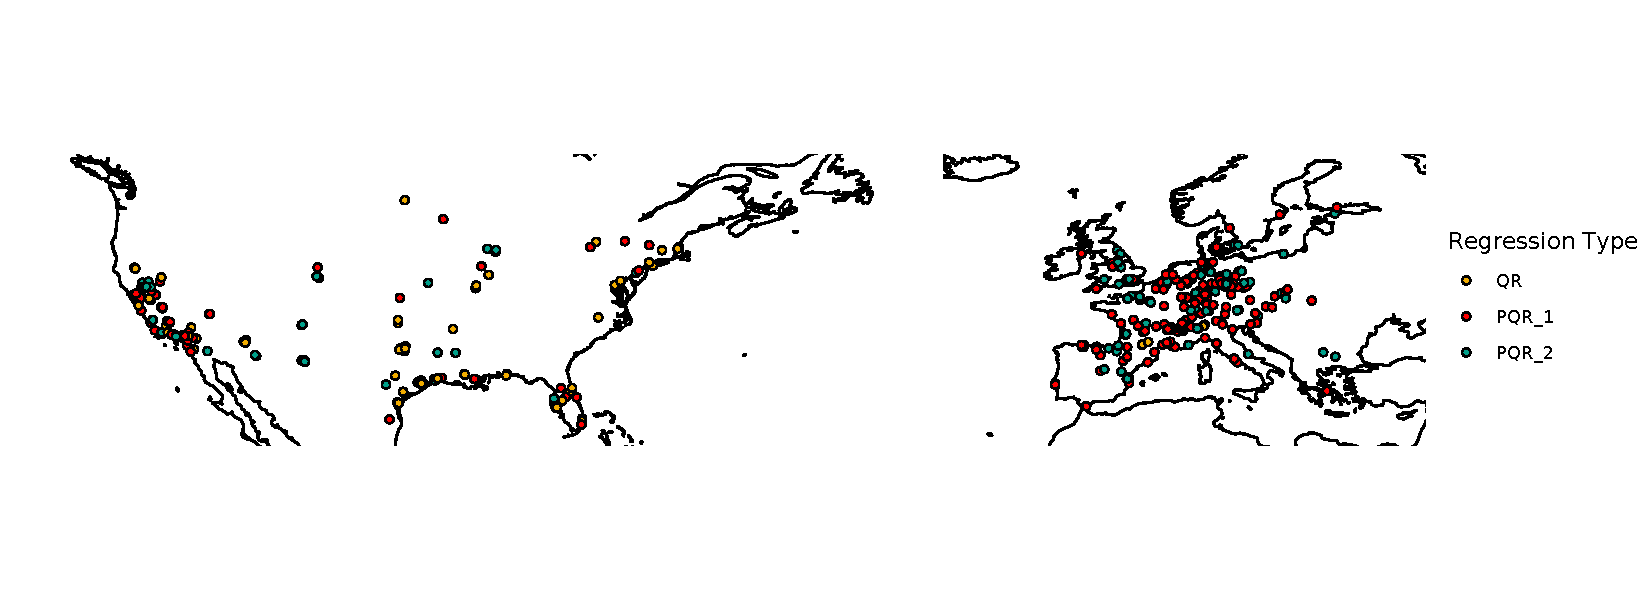
\includegraphics[width=\linewidth]{figures/si_figures/fS03_regression_type_map.pdf}
\caption{}
\label{si_fig:reg_map}
\end{sidewaysfigure}
\clearpage

%%%%%% slopes %%%%%%

\begin{sidewaysfigure}[p]
\centering
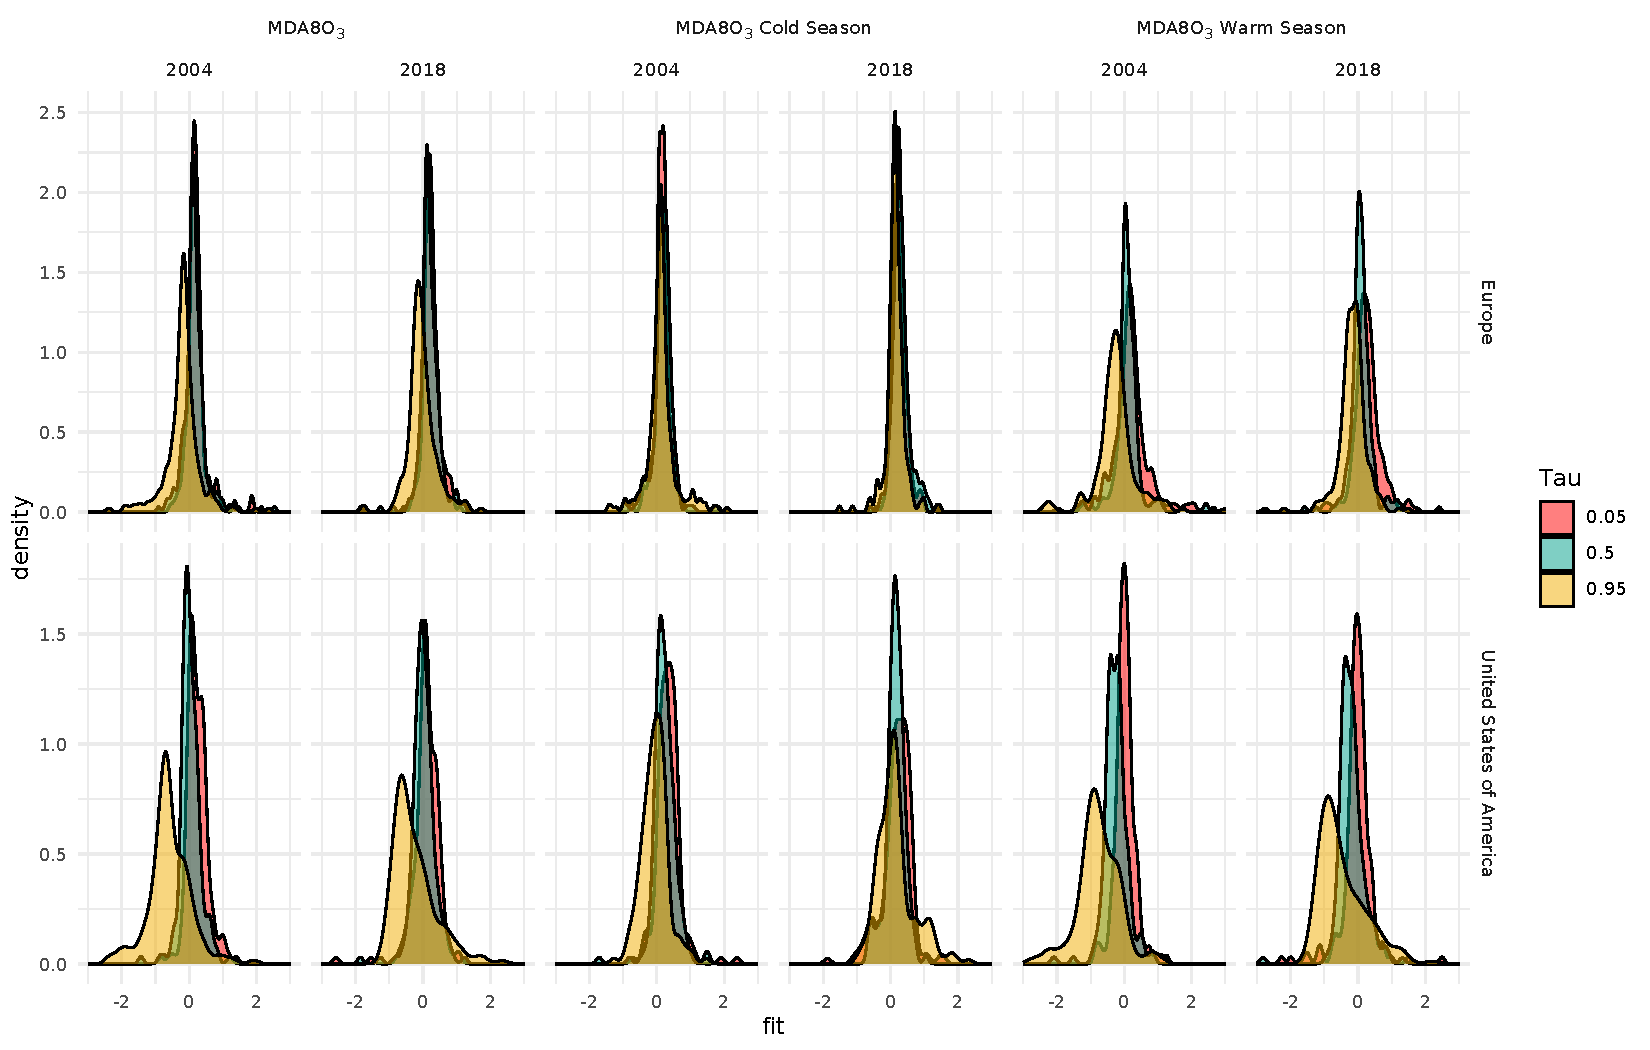
\includegraphics[width=\linewidth]{figures/si_figures/fS04_slope_density.pdf}
\caption{}
\label{si_fig:slope_density}
\end{sidewaysfigure}
\clearpage

%%%%%% arrow maps %%%%%%

\begin{figure}[p]
\centering
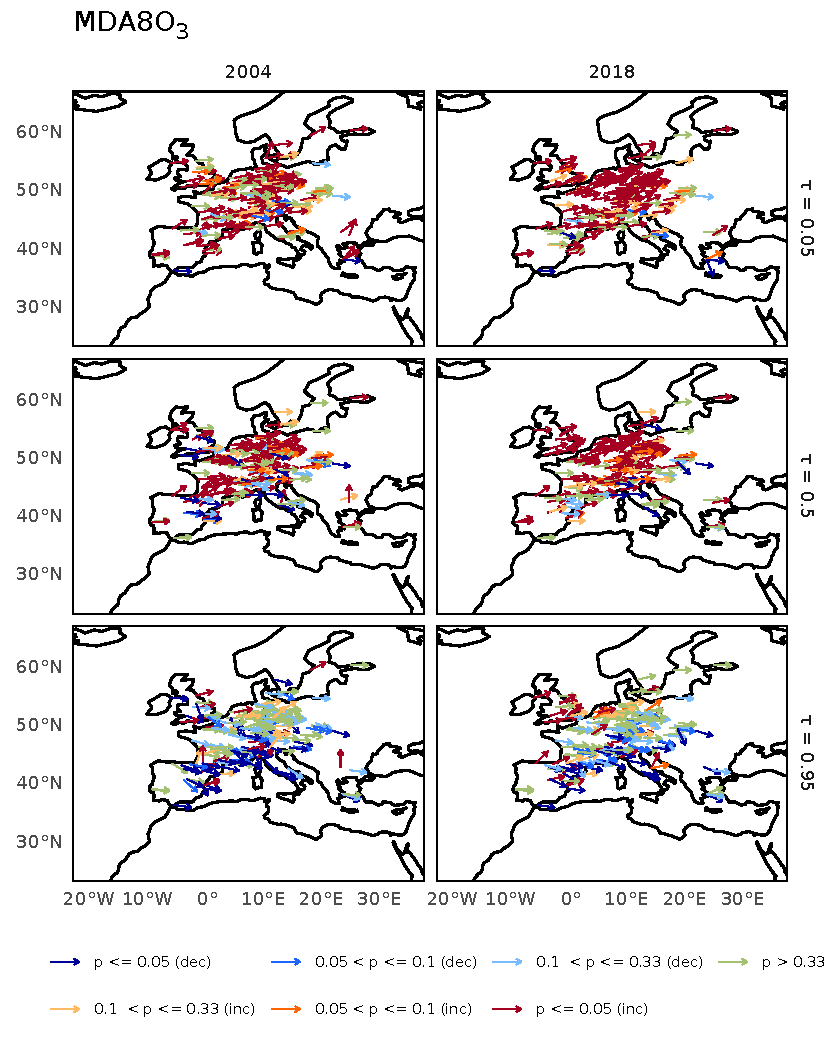
\includegraphics[height=0.9\textheight]{figures/si_figures/fS05_o3_map_mda8_all_eu_o3.pdf}
\caption{Trends in MDA8O\textsubscript{3} in Europe in 2004 and 2018. Trends are shown by an arrow where the angle between vertically up and horizontal corresponds to 2.5 - 0 ppbv / yr\textsuperscript{-1}, and between horizontal and vertically down corresponds to 0 - -2.5 ppbv / yr\textsuperscript{-1}. The few trends that have a magnitude greater than 2.5 ppbv have been clamped. Colour corresponds to the direction and significant of the trend.}
\label{si_fig:o3_map_eu_mda8}
\end{figure}
\clearpage

\begin{figure}[p]
\centering
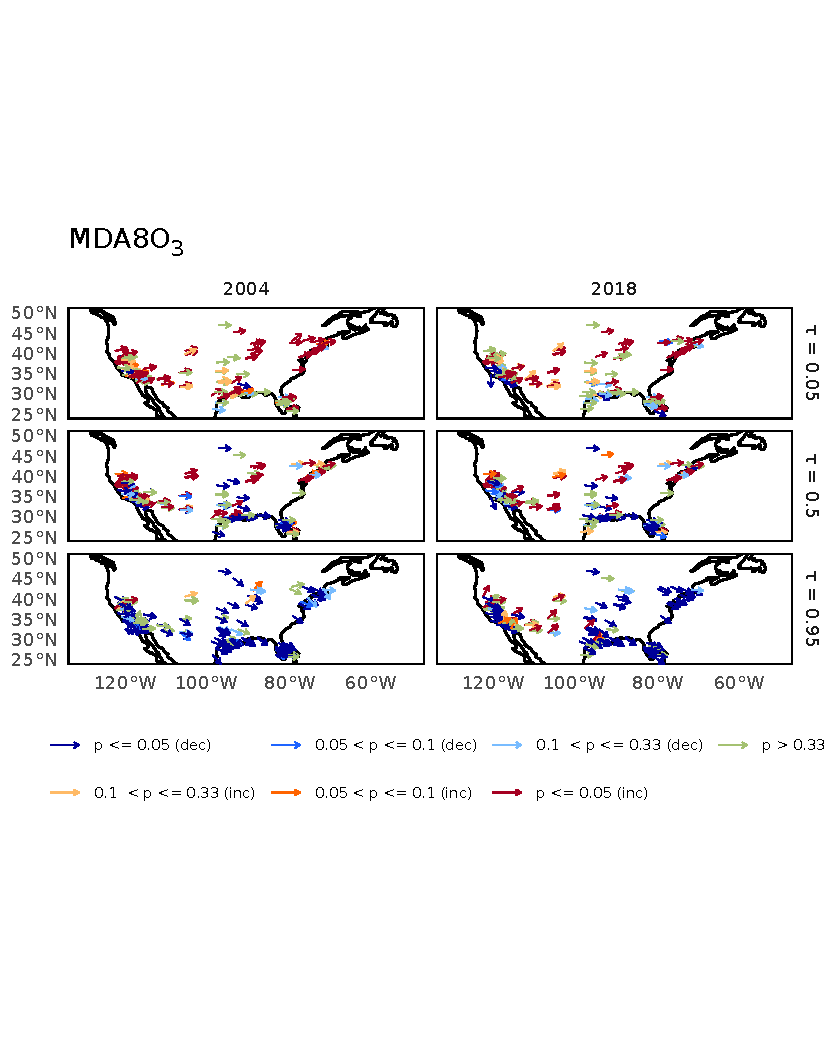
\includegraphics[height=0.9\textheight]{figures/si_figures/fS06_o3_map_mda8_all_us_o3.pdf}
\caption{Trends in MDA8O\textsubscript{3} in the United States of America in 2004 and 2018. Trends are shown by an arrow where the angle between vertically up and horizontal corresponds to 2.5 - 0 ppbv / yr\textsuperscript{-1}, and between horizontal and vertically down corresponds to 0 - -2.5 ppbv / yr\textsuperscript{-1}. The few trends that have a magnitude greater than 2.5 ppbv have been clamped. Colour corresponds to the direction and significant of the trend.}
\label{si_fig:o3_map_us_mda8}
\end{figure}
\clearpage

\begin{figure}[p]
\centering
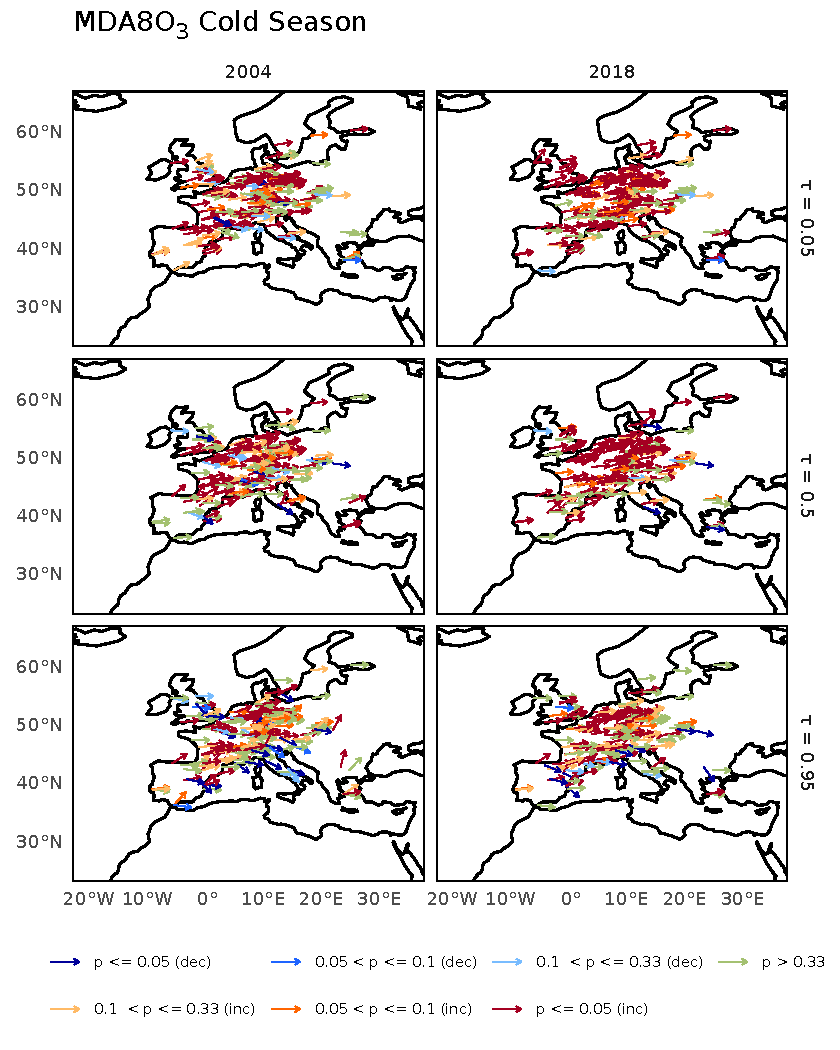
\includegraphics[height=0.9\textheight]{figures/si_figures/fS07_o3_map_mda8_cold_eu_o3.pdf}
\caption{Trends in cold season MDA8O\textsubscript{3} in Europe in 2004 and 2018. Trends are shown by an arrow where the angle between vertically up and horizontal corresponds to 2.5 - 0 ppbv / yr\textsuperscript{-1}, and between horizontal and vertically down corresponds to 0 - -2.5 ppbv / yr\textsuperscript{-1}. The few trends that have a magnitude greater than 2.5 ppbv have been clamped. Colour corresponds to the direction and significant of the trend.}
\label{si_fig:o3_map_eu_mda8_cold}
\end{figure}
\clearpage

\begin{figure}[p]
\centering
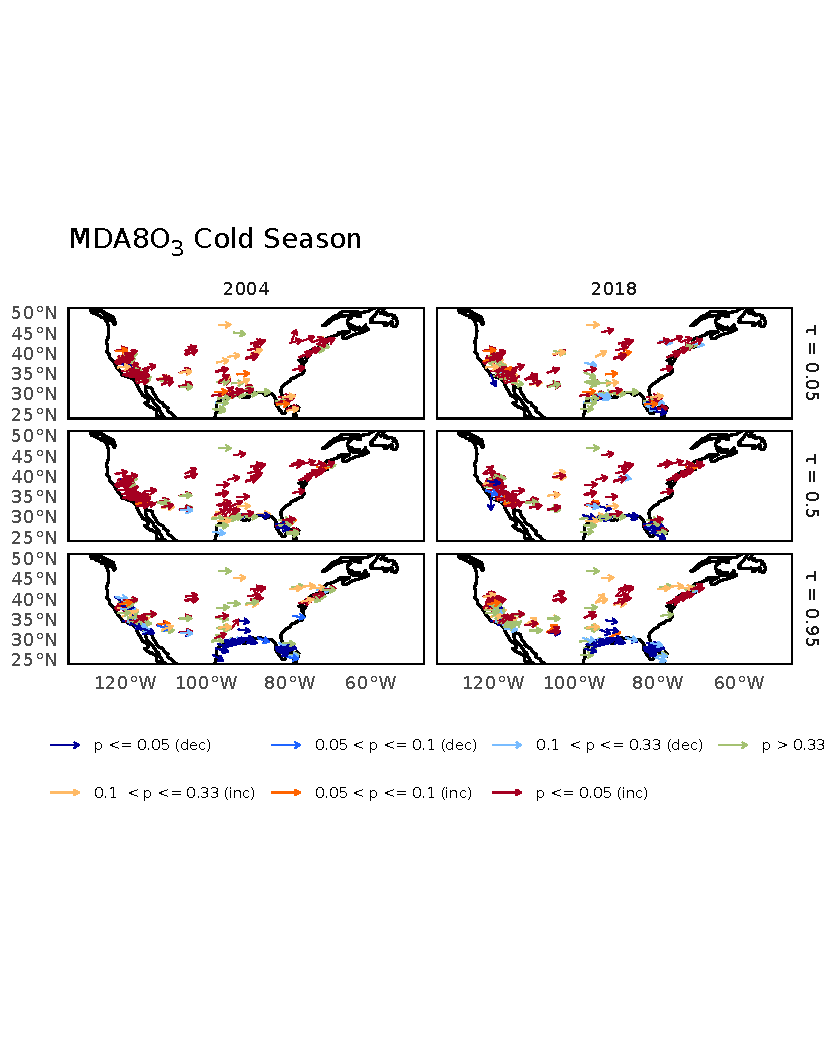
\includegraphics[height=0.9\textheight]{figures/si_figures/fS08_o3_map_mda8_cold_us_o3.pdf}
\caption{Trends in cold season MDA8O\textsubscript{3} in the United States of America in 2004 and 2018. Trends are shown by an arrow where the angle between vertically up and horizontal corresponds to 2.5 - 0 ppbv / yr\textsuperscript{-1}, and between horizontal and vertically down corresponds to 0 - -2.5 ppbv / yr\textsuperscript{-1}. The few trends that have a magnitude greater than 2.5 ppbv have been clamped. Colour corresponds to the direction and significant of the trend.}
\label{si_fig:o3_map_us_mda8_cold}
\end{figure}
\clearpage


%%%%%% metric maps - Europe %%%%%%
\begin{sidewaysfigure}[p]
\centering
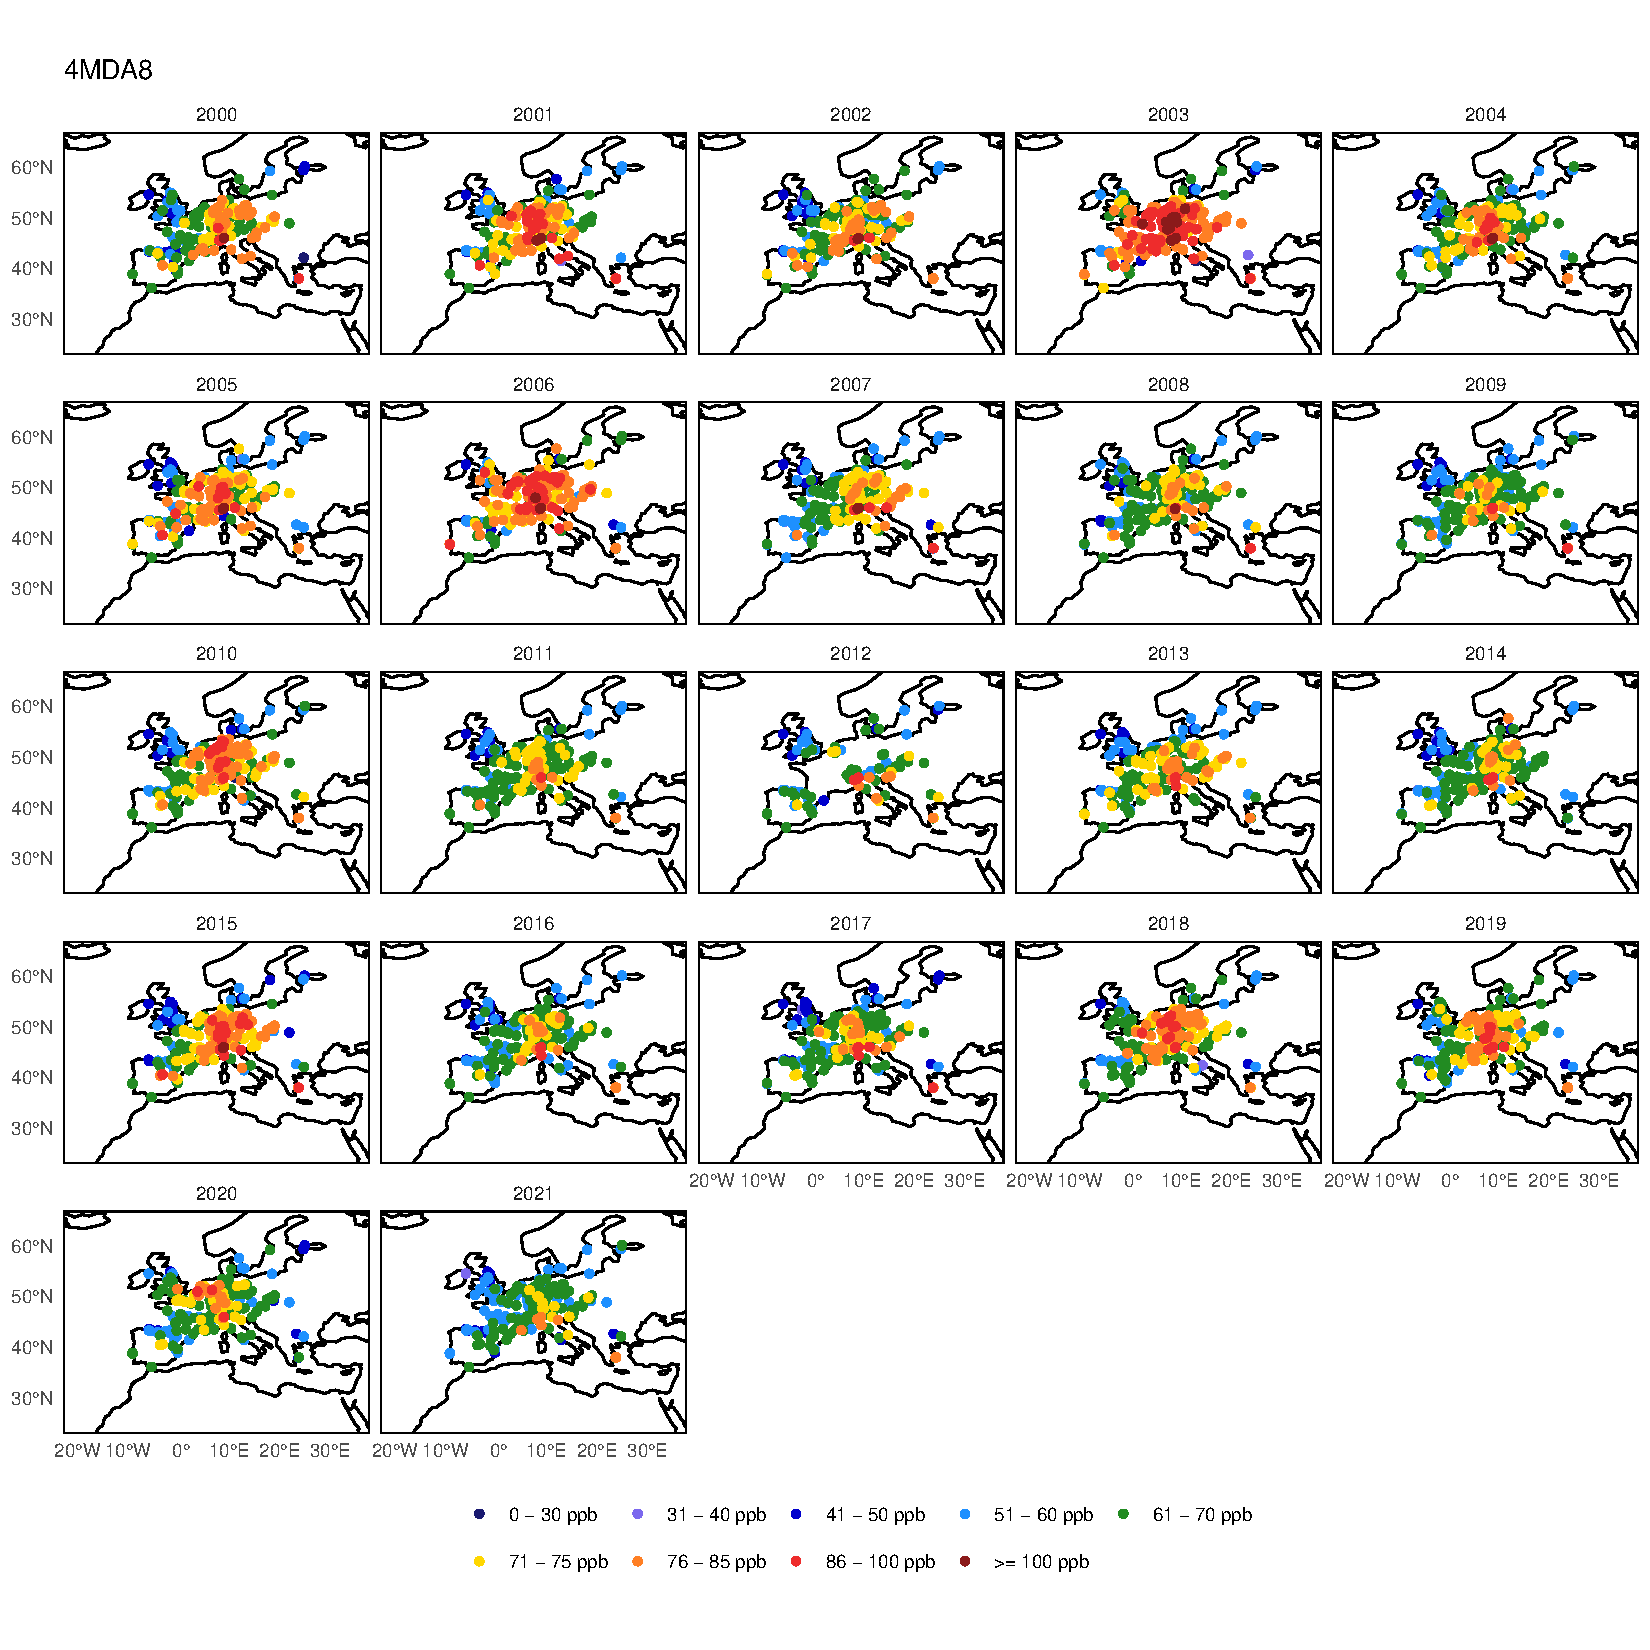
\includegraphics[height=0.9\textheight]{figures/si_figures/fS09_metric_map_Europe_4MDA8.pdf}
\caption{}
\label{si_fig:metric_map_eu_4MDA8}
\end{sidewaysfigure}
\clearpage

\begin{sidewaysfigure}[p]
\centering
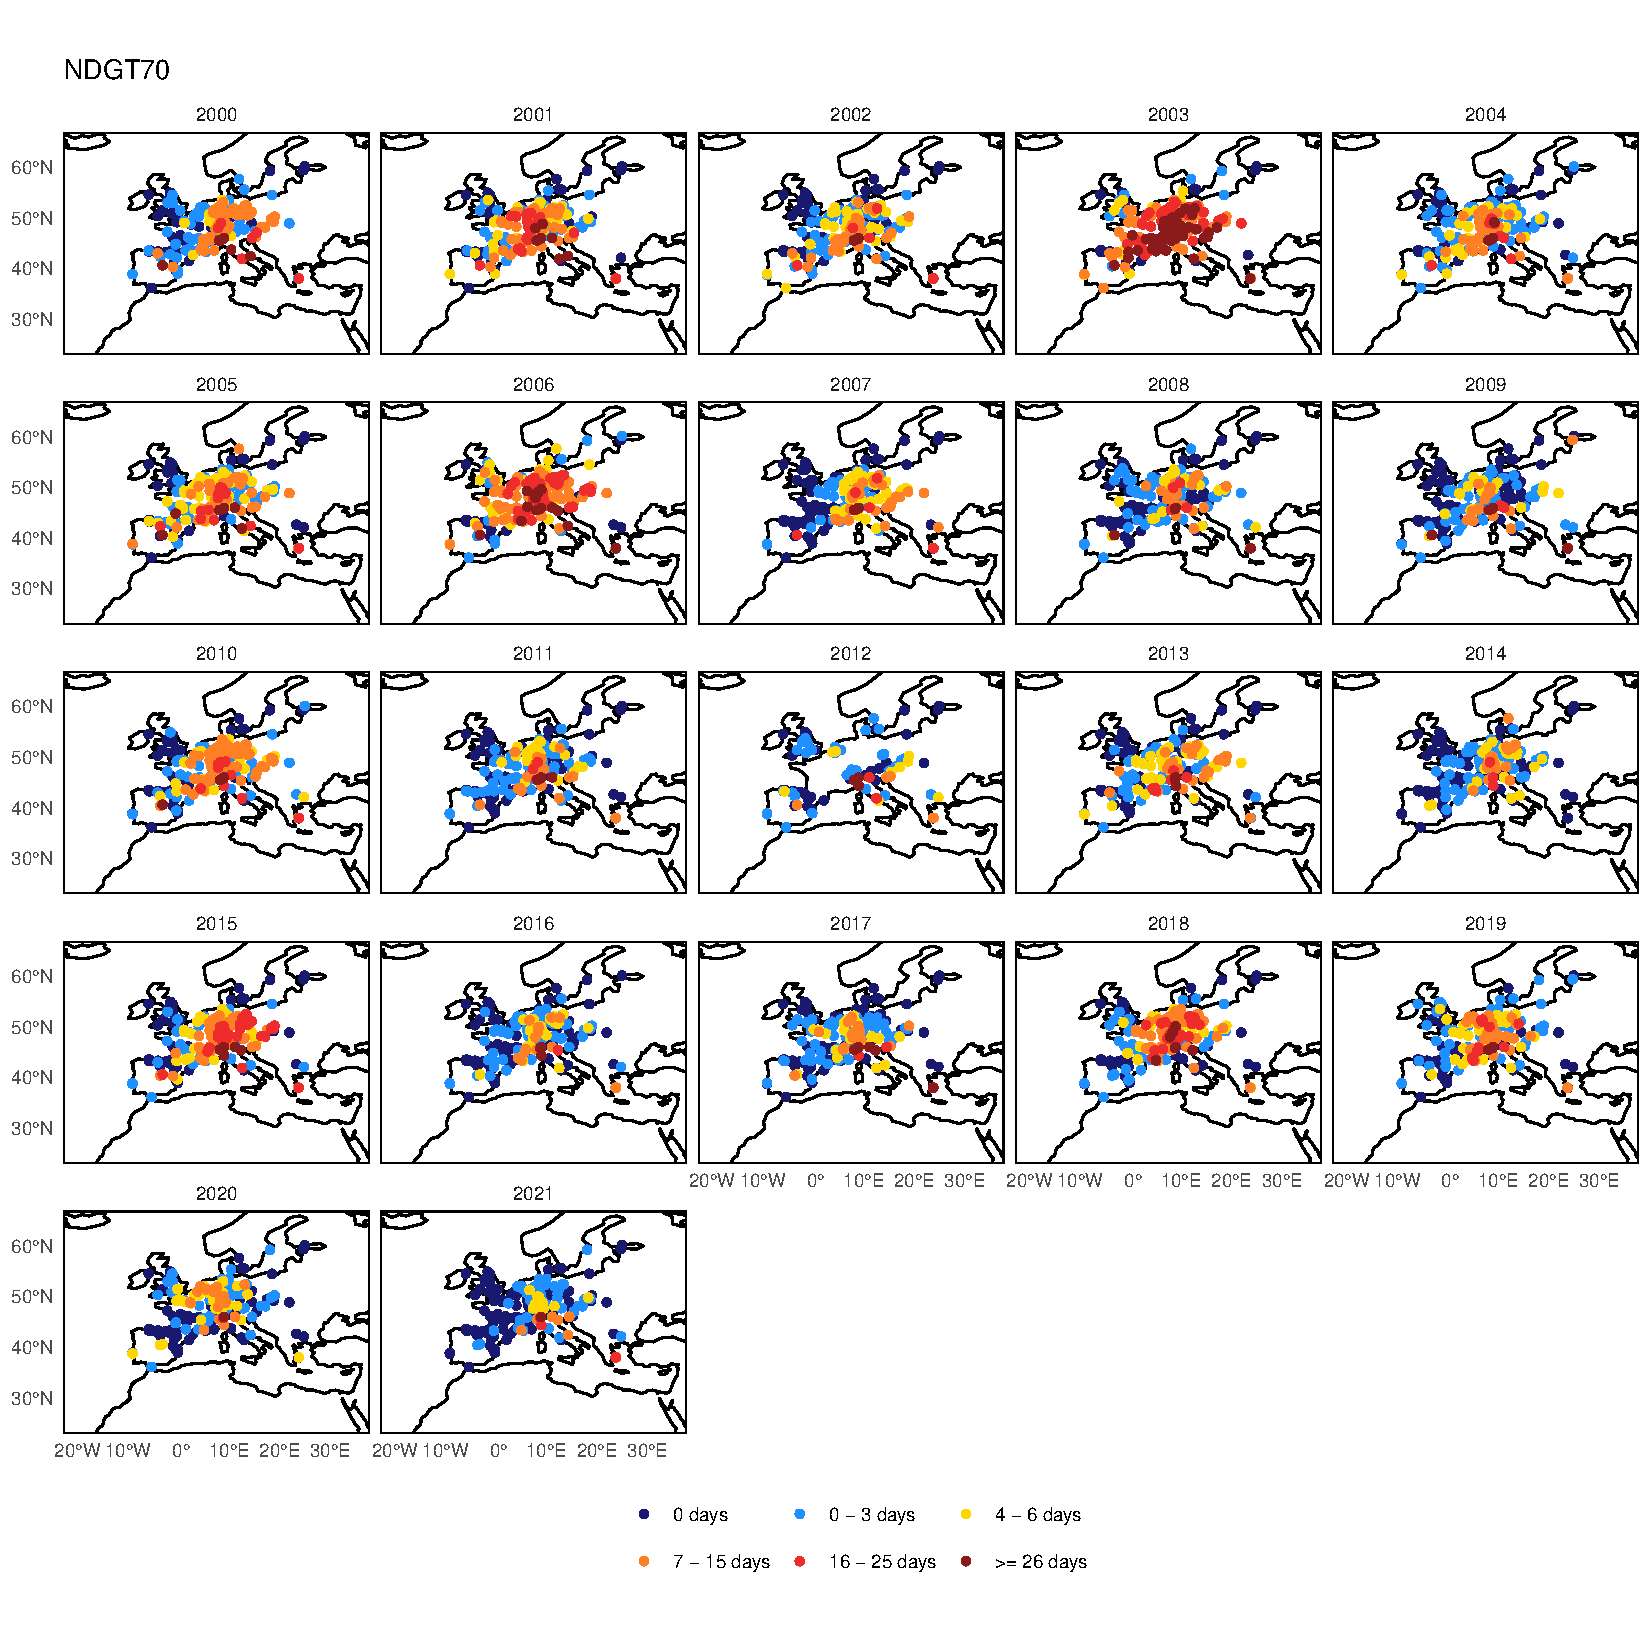
\includegraphics[height=0.9\textheight]{figures/si_figures/fS10_metric_map_Europe_NDGT70.pdf}
\caption{}
\label{si_fig:metric_map_eu_NDGT70}
\end{sidewaysfigure}
\clearpage


\begin{sidewaysfigure}[p]
\centering
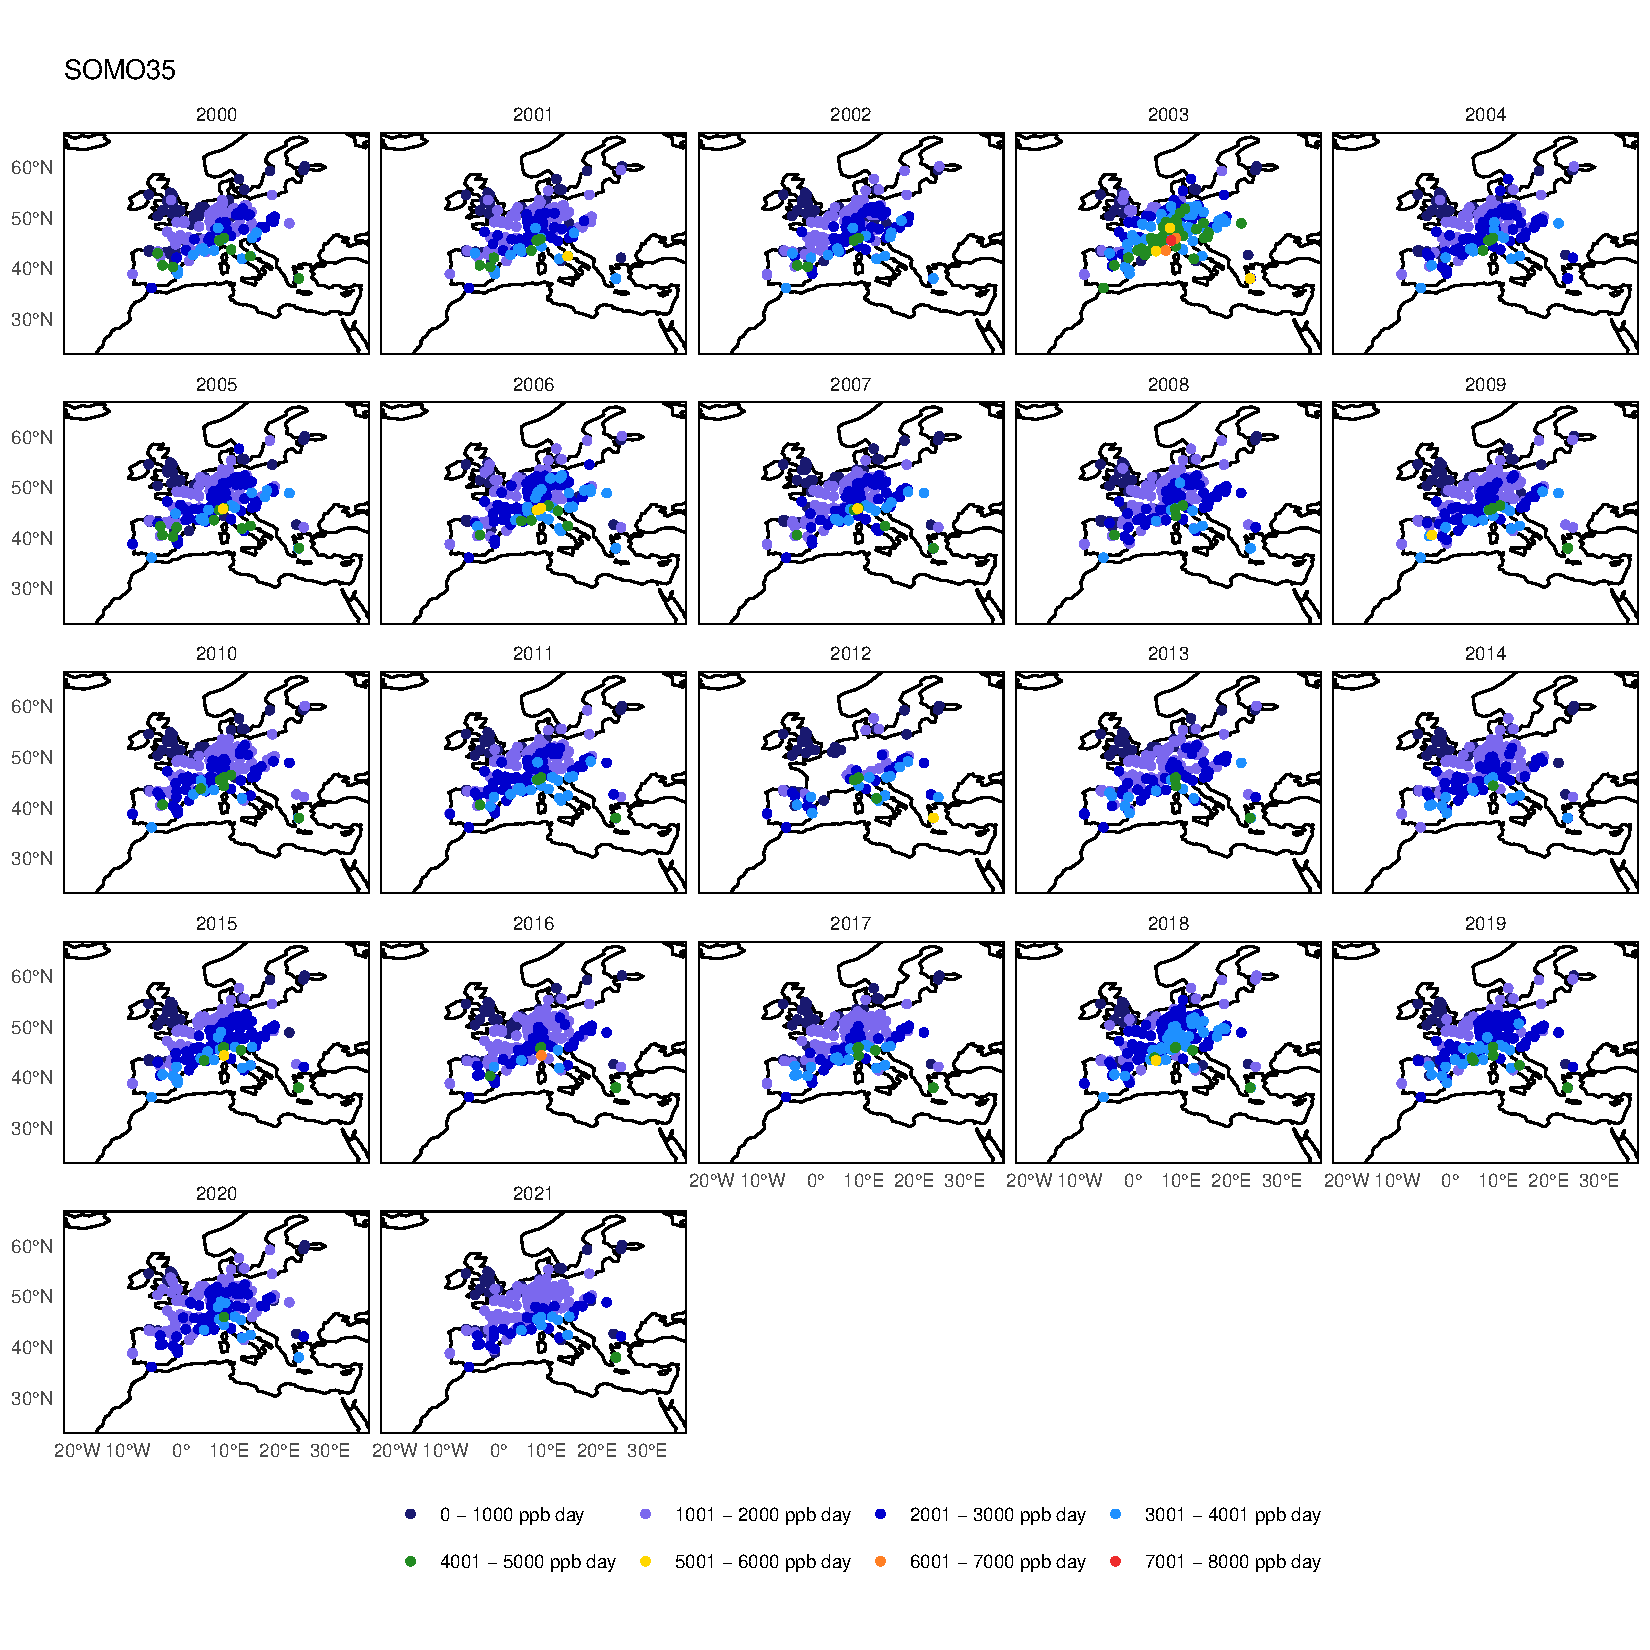
\includegraphics[height=0.9\textheight]{figures/si_figures/fS11_metric_map_Europe_SOMO35.pdf}
\caption{}
\label{si_fig:metric_map_eu_SOMO35}
\end{sidewaysfigure}
\clearpage

\begin{sidewaysfigure}[p]
\centering
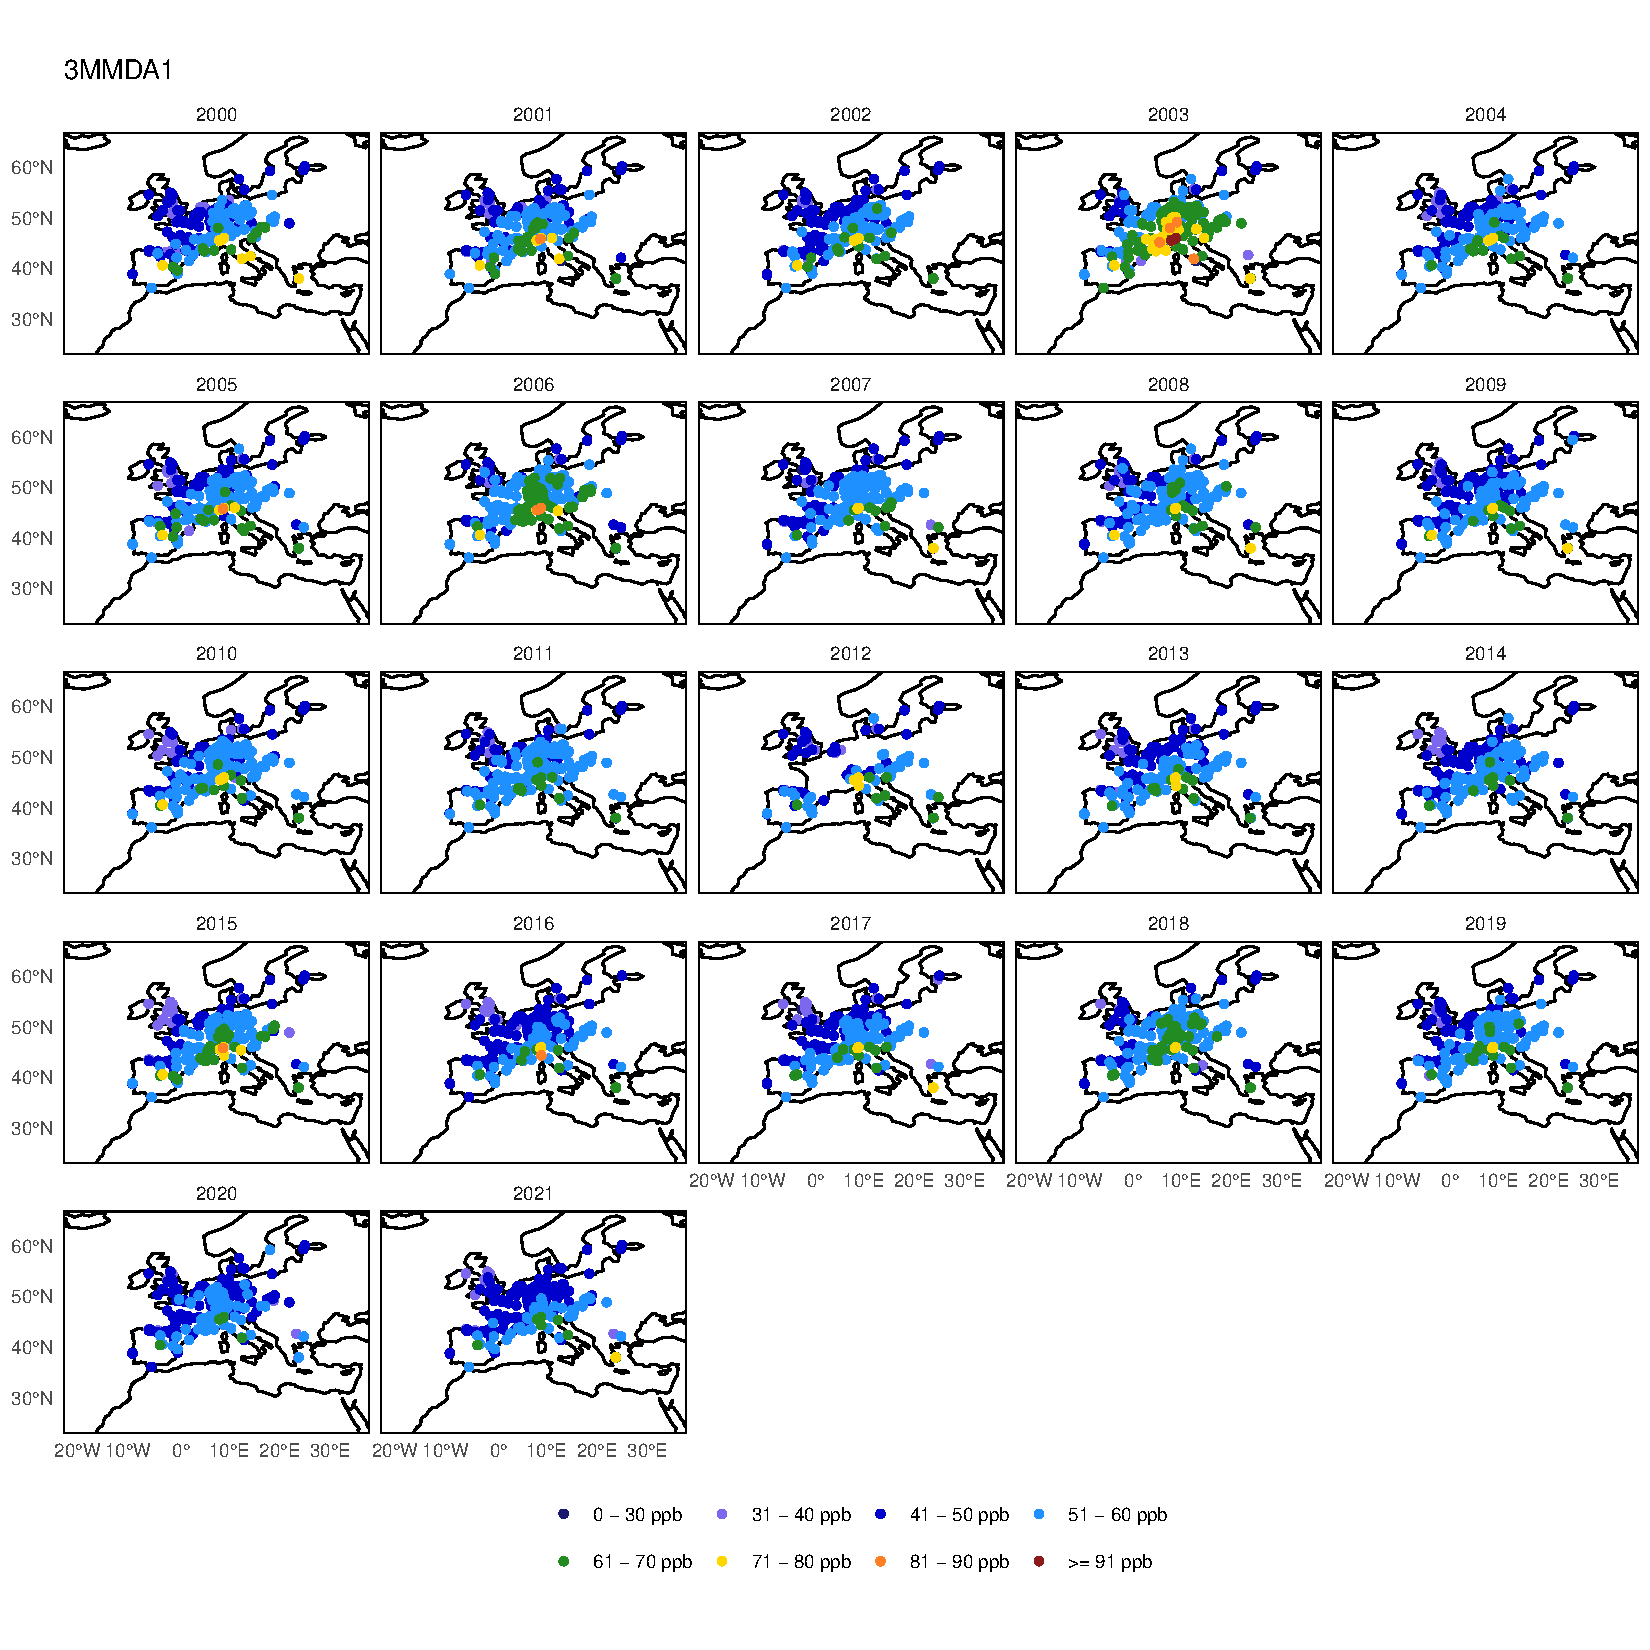
\includegraphics[height=0.9\textheight]{figures/si_figures/fS12_metric_map_Europe_3MMDA1.pdf}
\caption{}
\label{si_fig:metric_map_eu_3MMDA1}
\end{sidewaysfigure}
\clearpage

\begin{sidewaysfigure}[p]
\centering
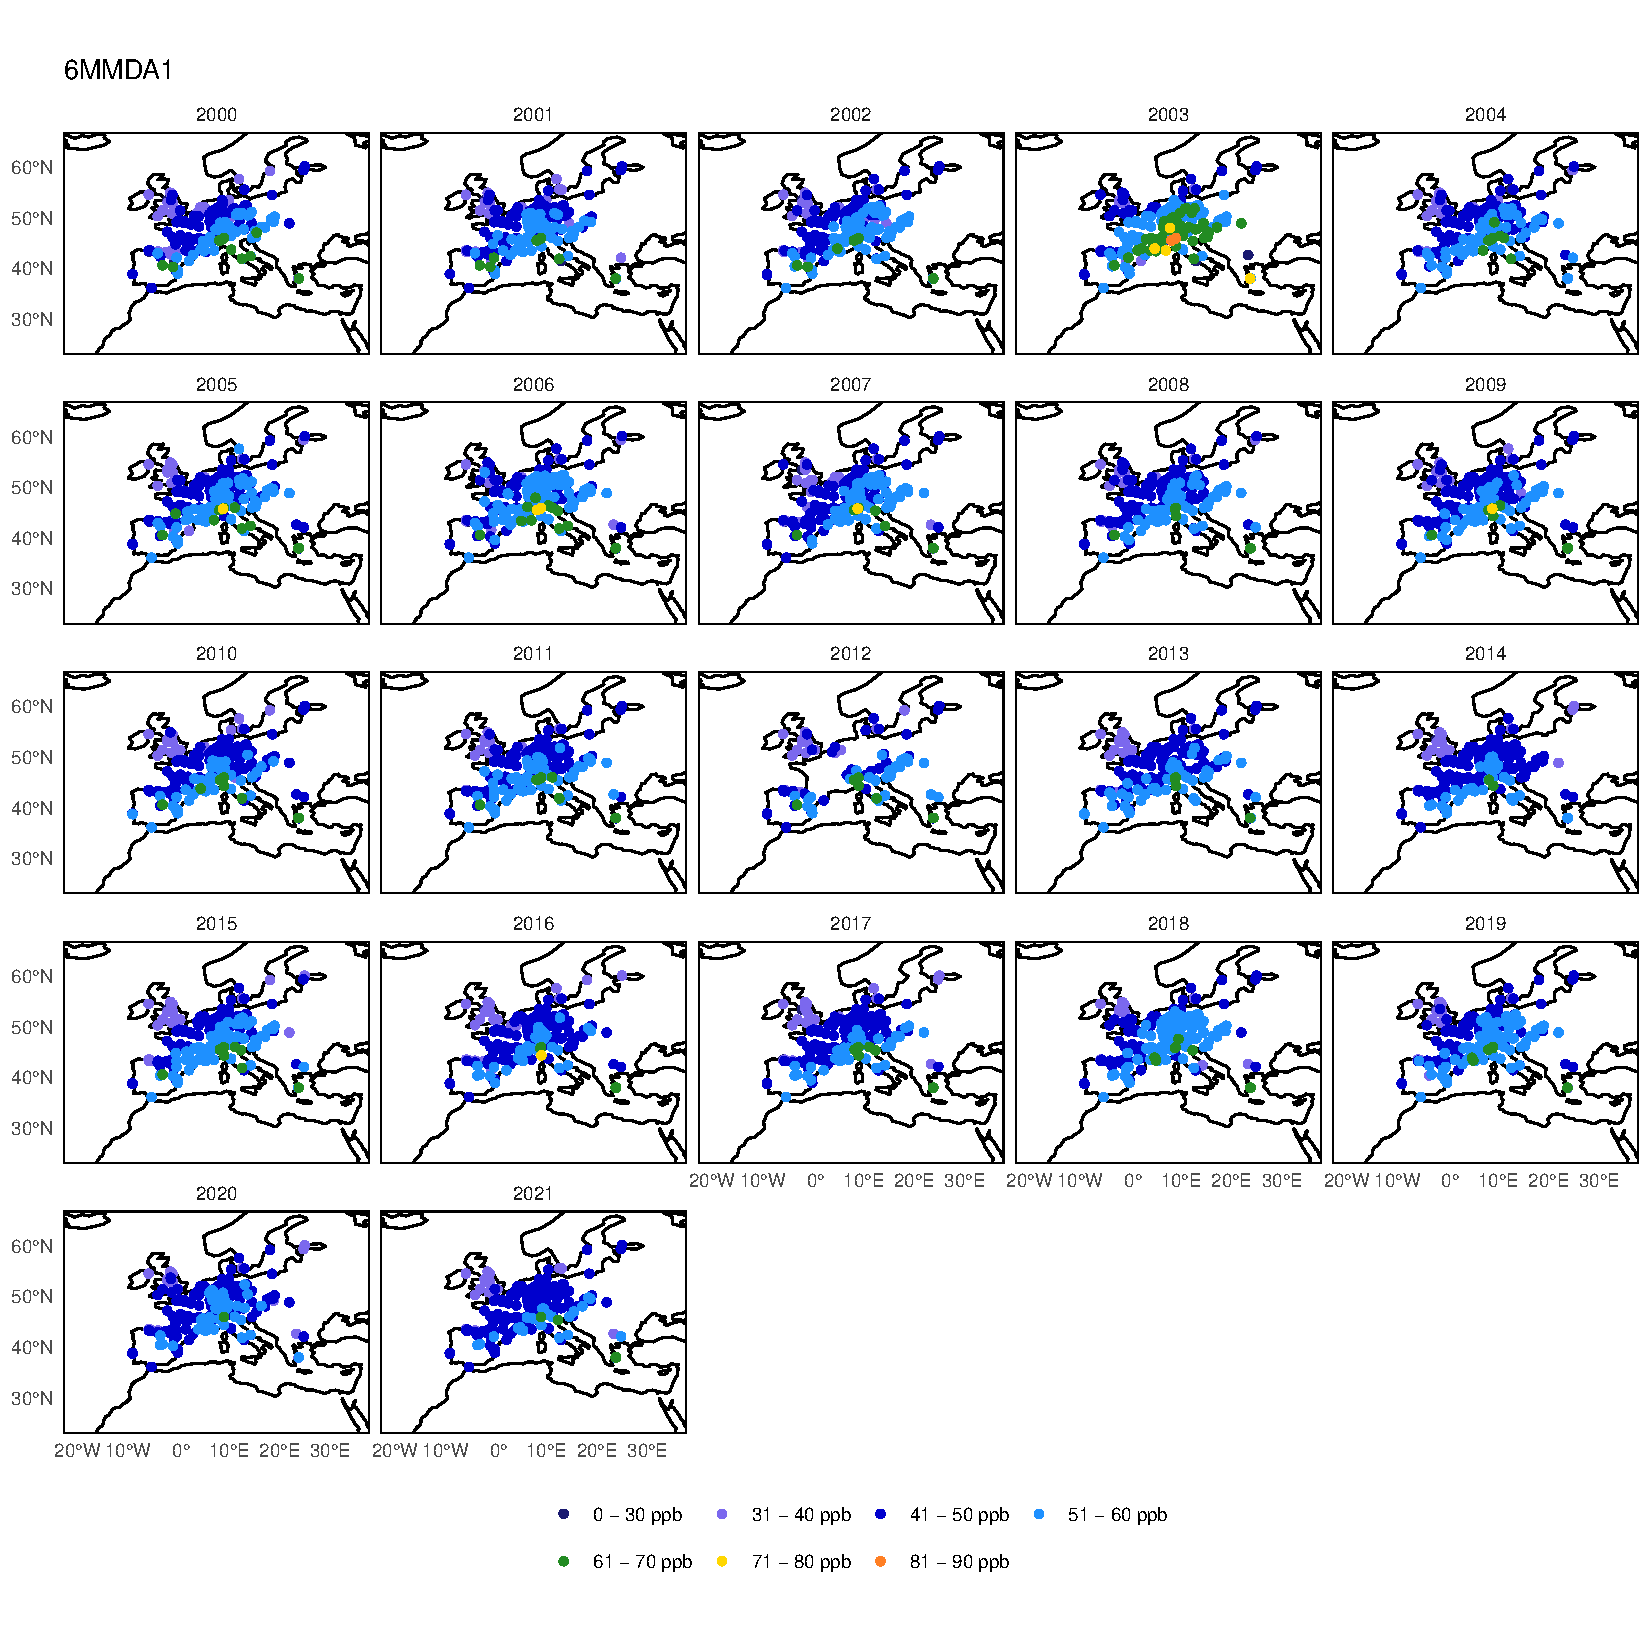
\includegraphics[height=0.9\textheight]{figures/si_figures/fS13_metric_map_Europe_6MMDA1.pdf}
\caption{}
\label{si_fig:metric_map_eu_6MMDA1}
\end{sidewaysfigure}
\clearpage

\begin{sidewaysfigure}[p]
\centering
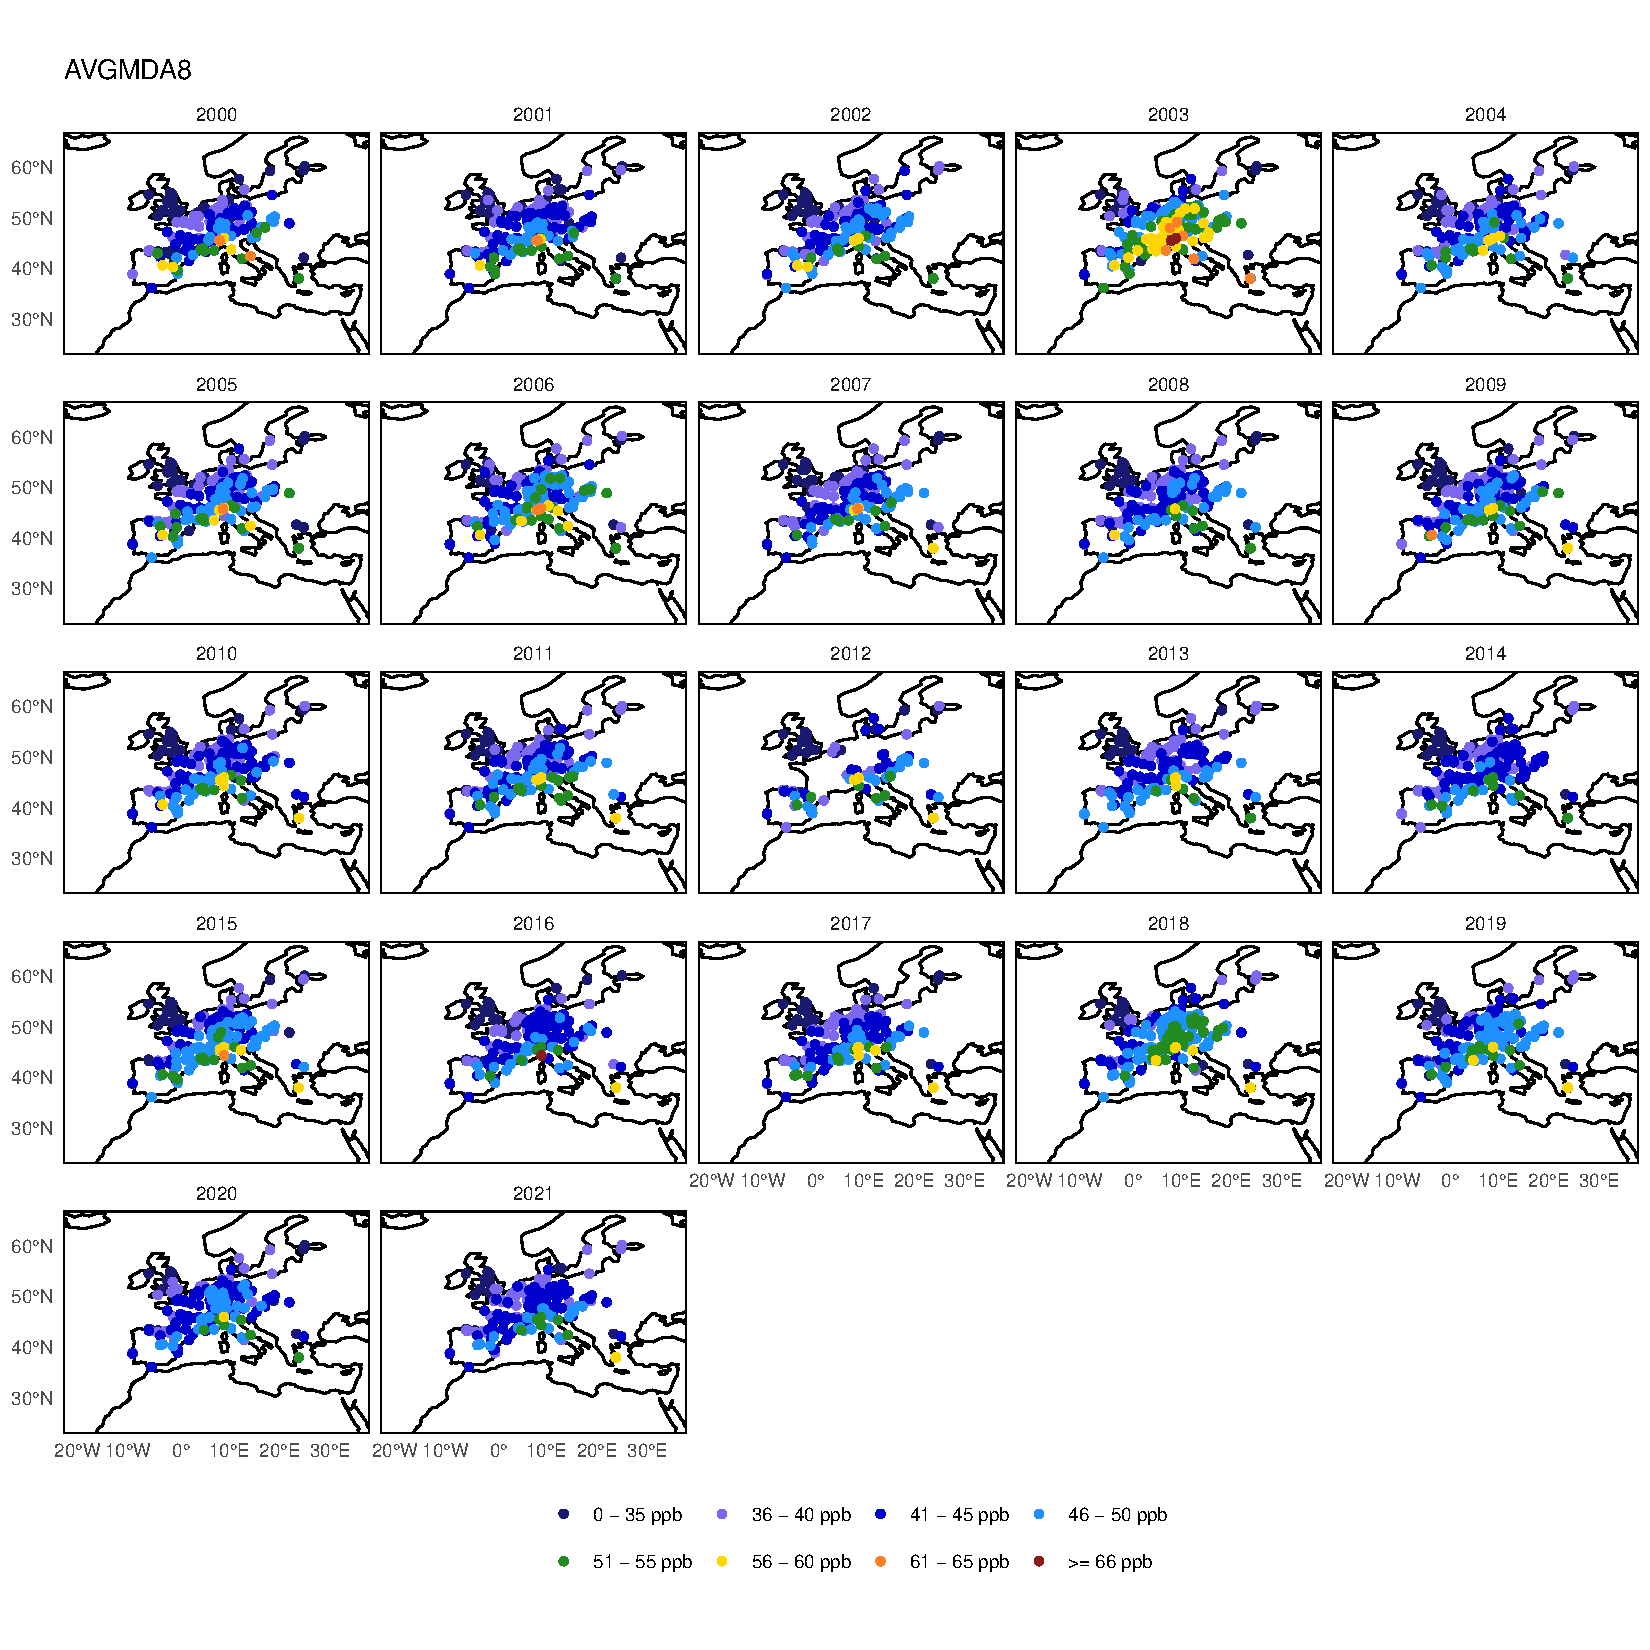
\includegraphics[height=0.9\textheight]{figures/si_figures/fS14_metric_map_Europe_AVGMDA8.pdf}
\caption{}
\label{si_fig:metric_map_eu_AVGMDA8}
\end{sidewaysfigure}
\clearpage

%%%%%% metric maps - USA %%%%%%

\begin{sidewaysfigure}[p]
\centering
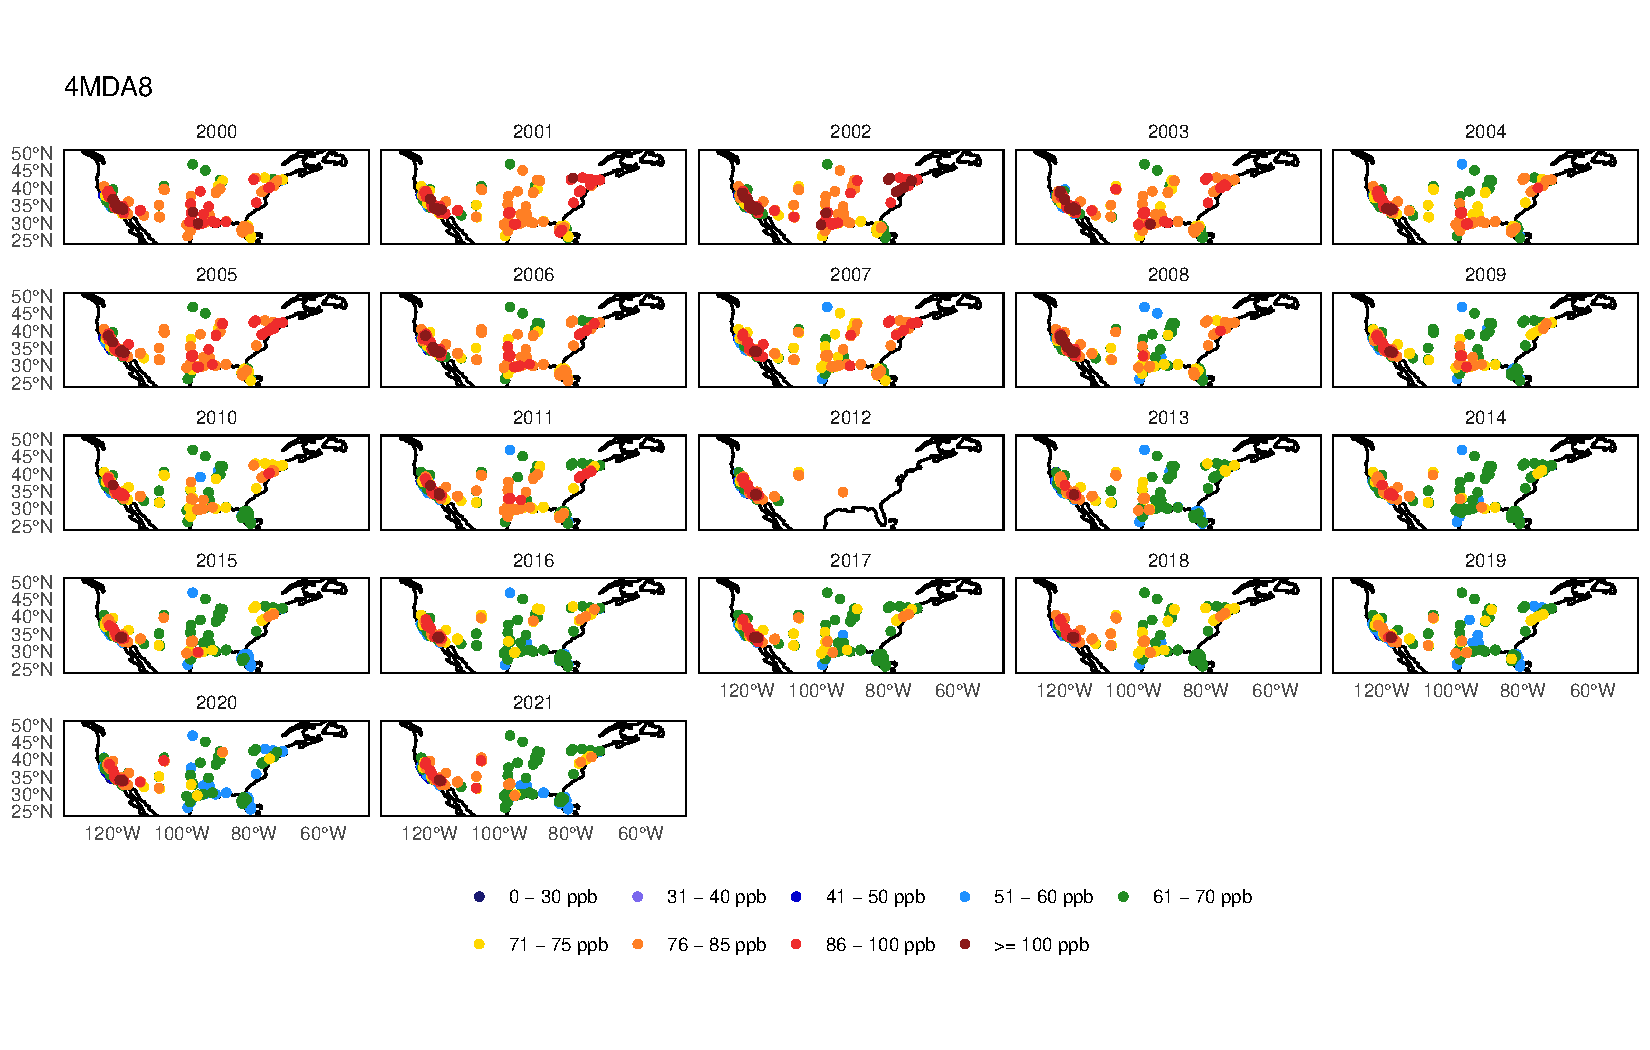
\includegraphics[height=0.75\textheight]{figures/si_figures/fS15_metric_map_United-States-of-America_4MDA8.pdf}
\caption{}
\label{si_fig:metric_map_us_4MDA8}
\end{sidewaysfigure}
\clearpage

\begin{sidewaysfigure}[p]
\centering
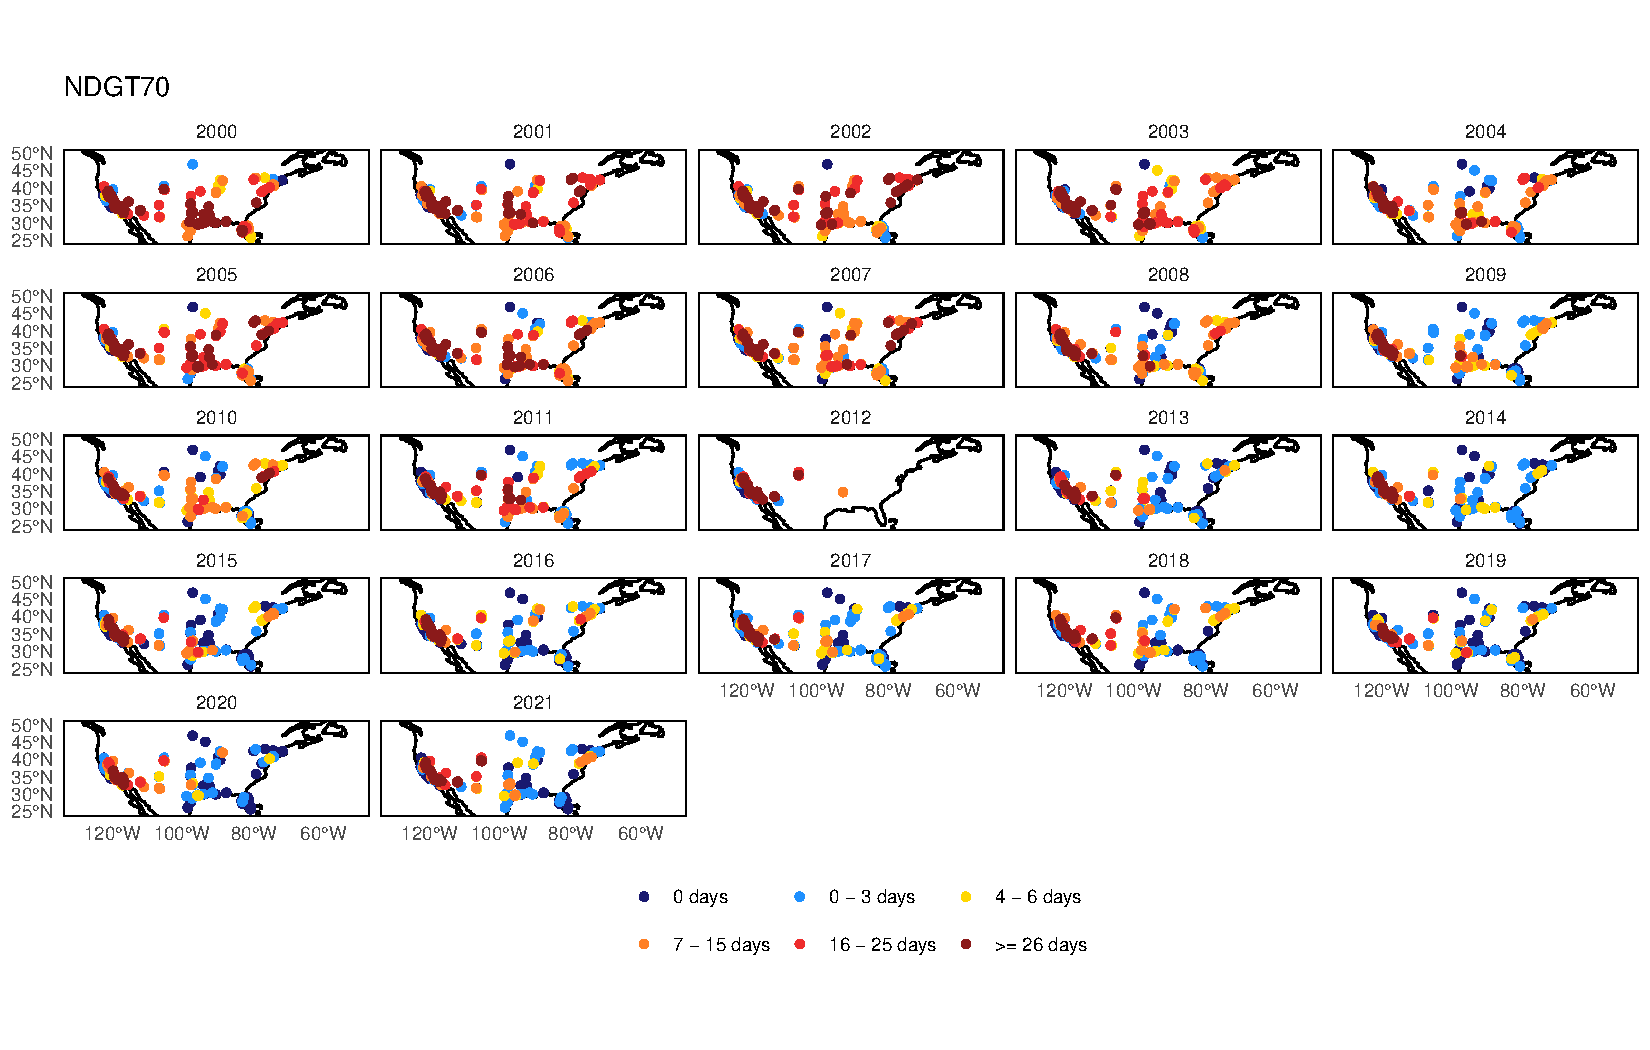
\includegraphics[height=0.75\textheight]{figures/si_figures/fS16_metric_map_United-States-of-America_NDGT70.pdf}
\caption{}
\label{si_fig:metric_map_us_NDGT70}
\end{sidewaysfigure}
\clearpage


\begin{sidewaysfigure}[p]
\centering
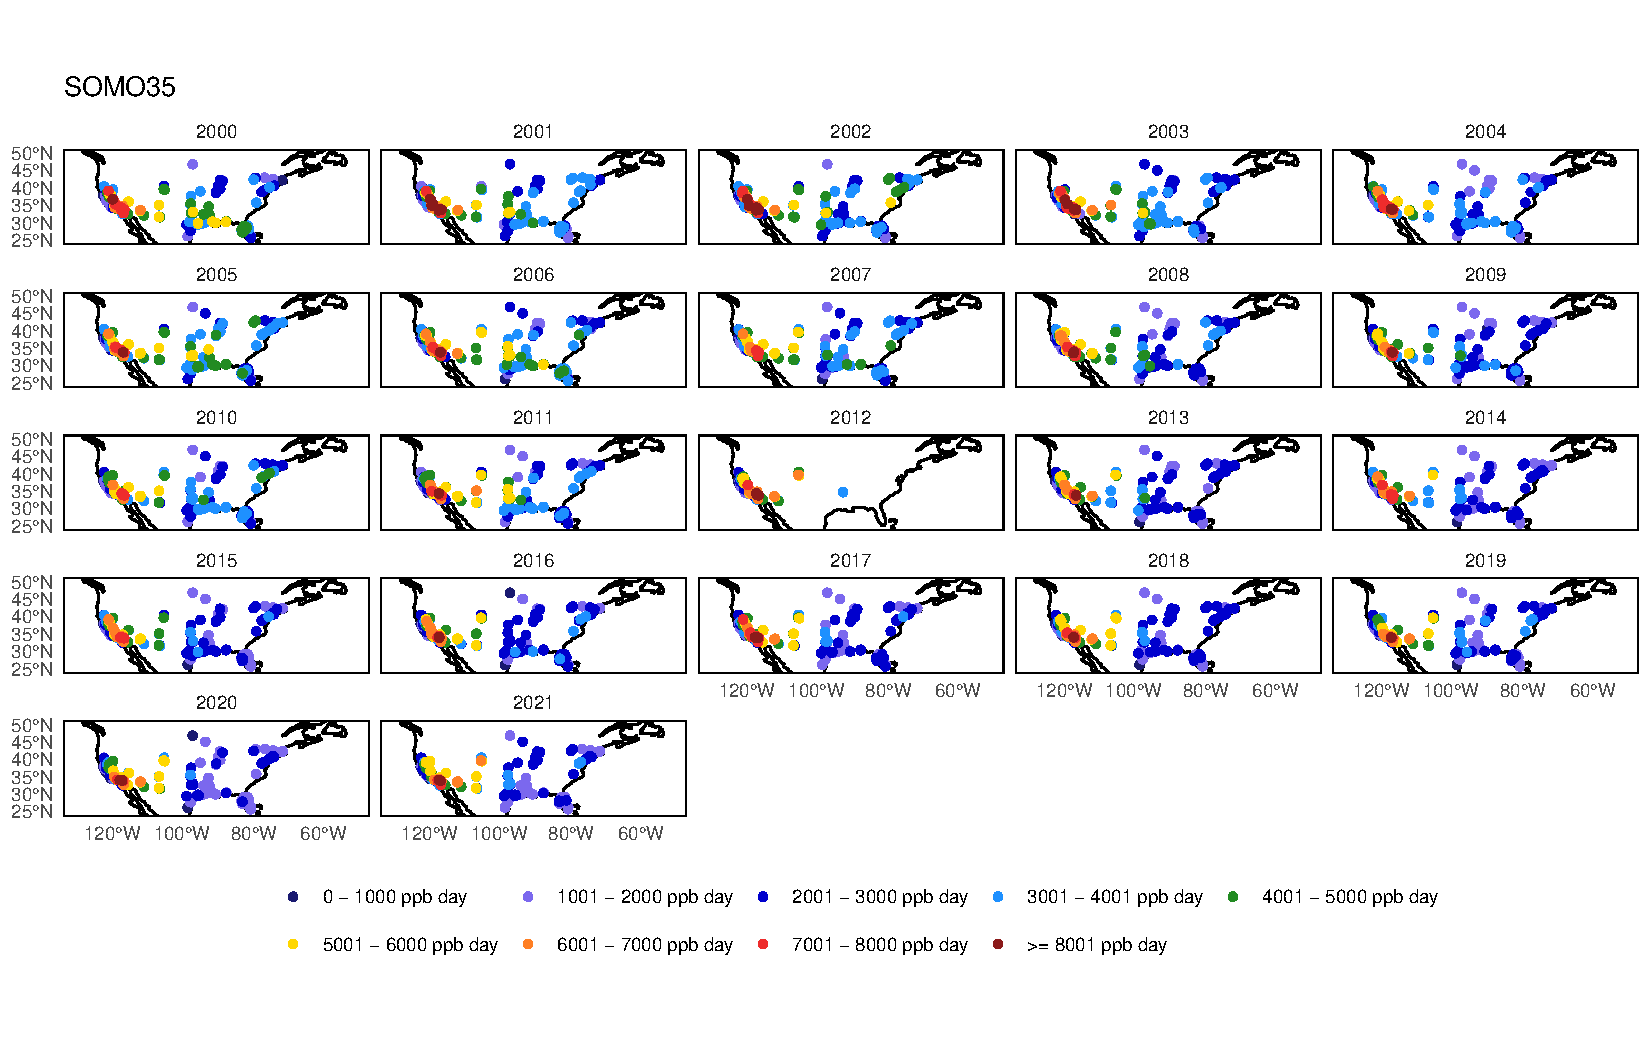
\includegraphics[height=0.75\textheight]{figures/si_figures/fS17_metric_map_United-States-of-America_SOMO35.pdf}
\caption{}
\label{si_fig:metric_map_us_SOMO35}
\end{sidewaysfigure}
\clearpage

\begin{sidewaysfigure}[p]
\centering
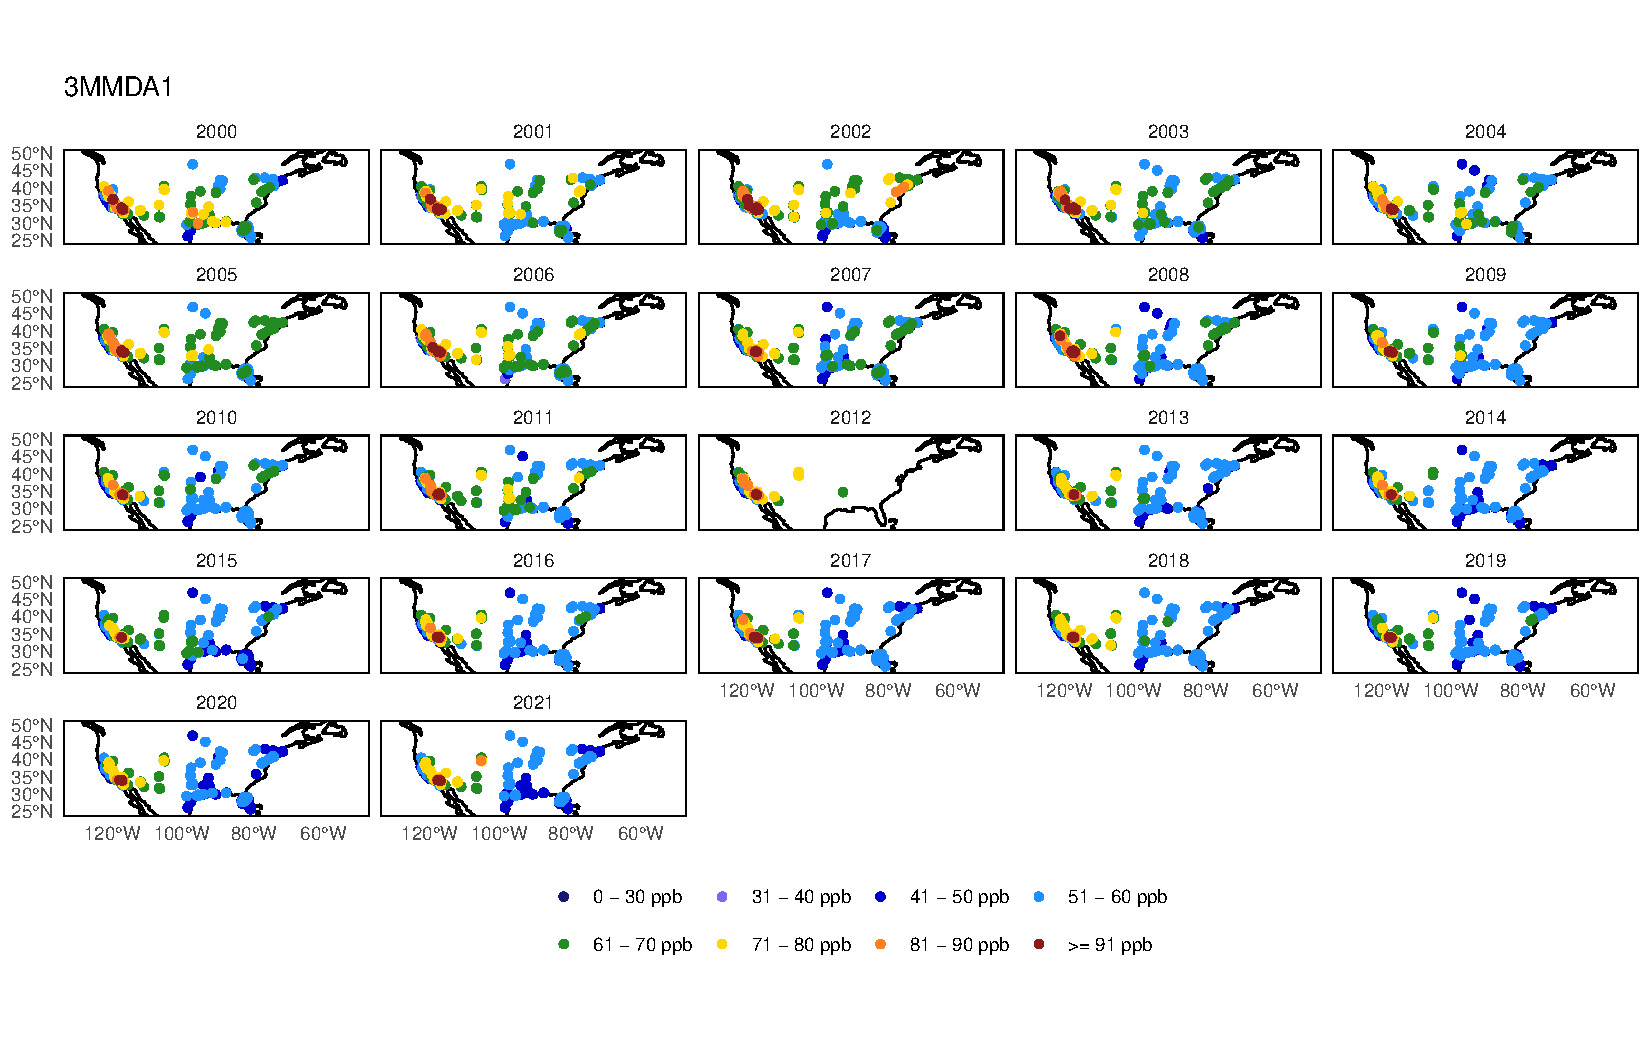
\includegraphics[height=0.75\textheight]{figures/si_figures/fS18_metric_map_United-States-of-America_3MMDA1.pdf}
\caption{}
\label{si_fig:metric_map_us_3MMDA1}
\end{sidewaysfigure}
\clearpage

\begin{sidewaysfigure}[p]
\centering
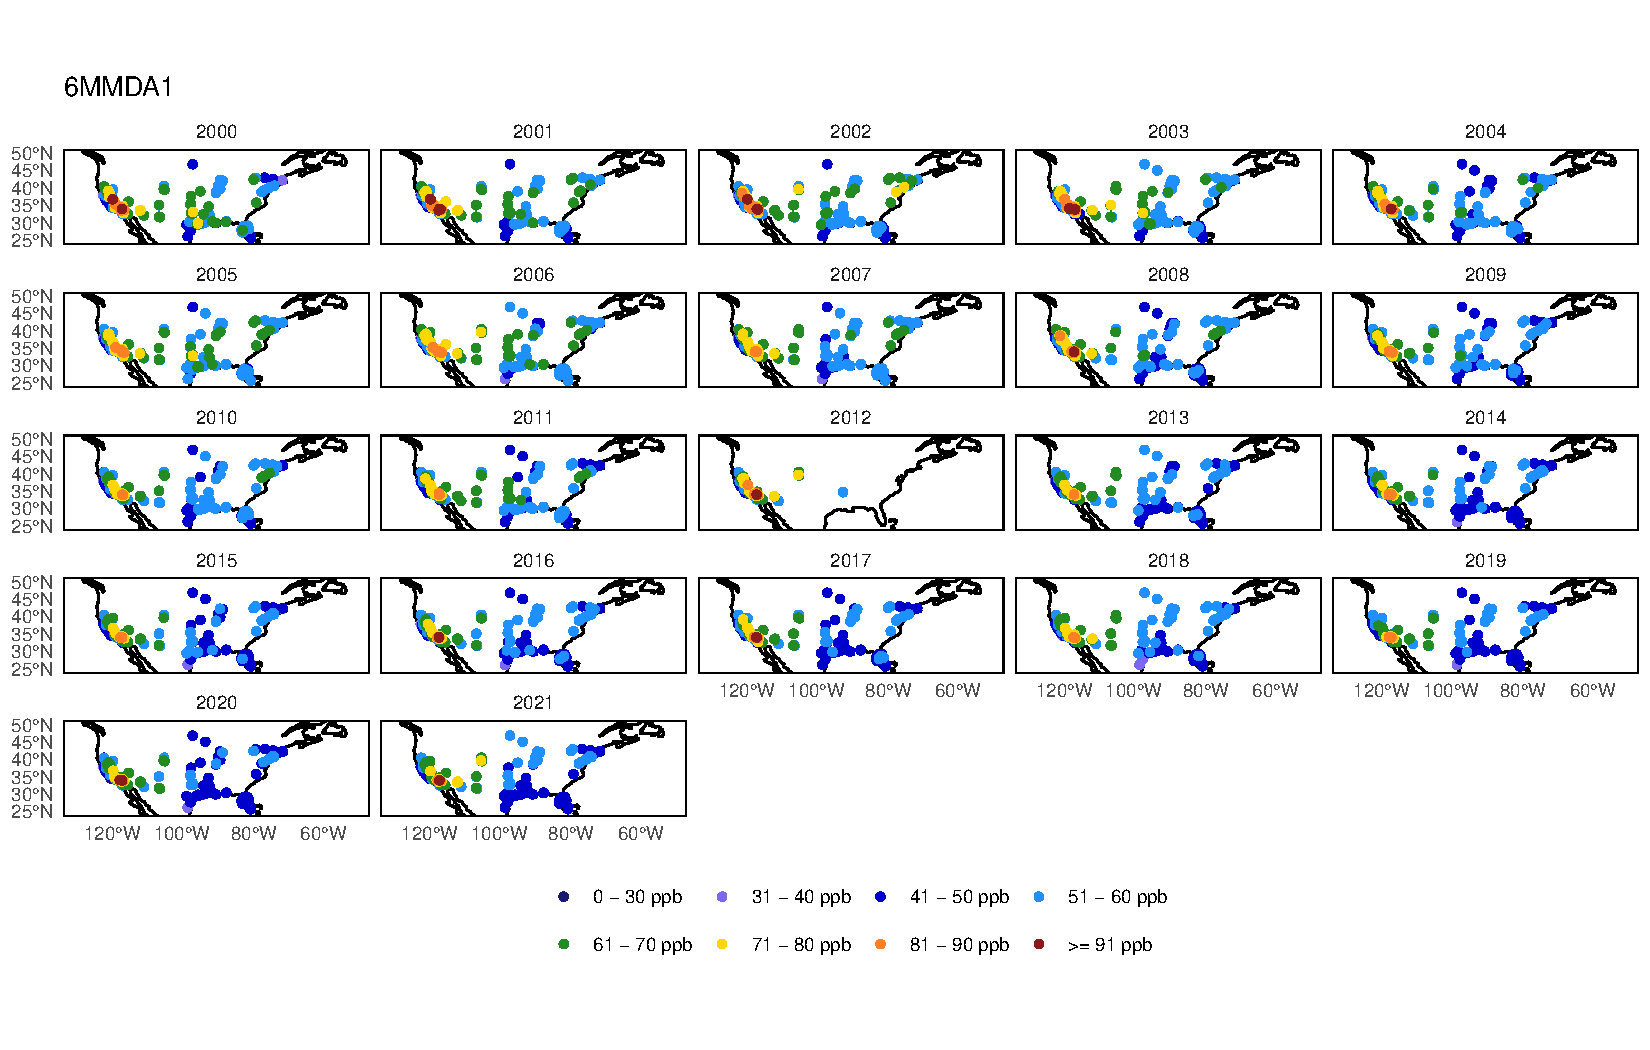
\includegraphics[height=0.75\textheight]{figures/si_figures/fS19_metric_map_United-States-of-America_6MMDA1.pdf}
\caption{}
\label{si_fig:metric_map_us_6MMDA1}
\end{sidewaysfigure}
\clearpage

\begin{sidewaysfigure}[p]
\centering
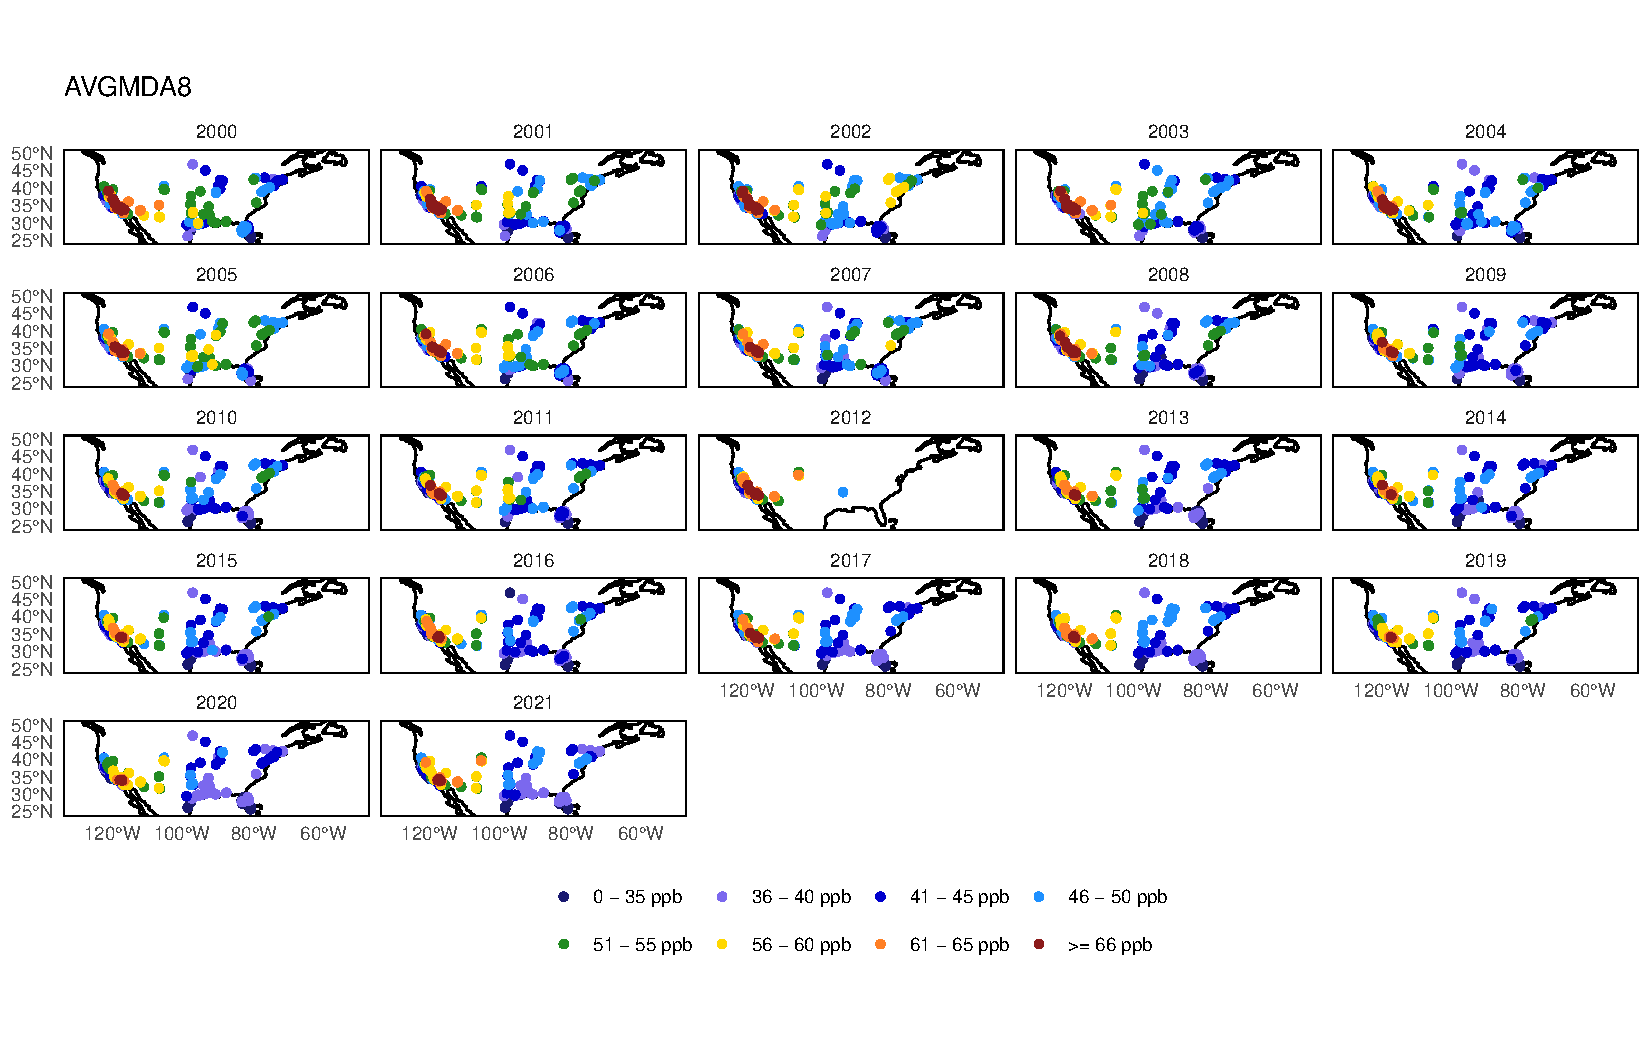
\includegraphics[height=0.75\textheight]{figures/si_figures/fS20_metric_map_United-States-of-America_AVGMDA8.pdf}
\caption{}
\label{si_fig:metric_map_us_AVGMDA8}
\end{sidewaysfigure}
\clearpage


%%%%%% 6MMDA1 %%%%%%

\begin{figure}[p]
\centering
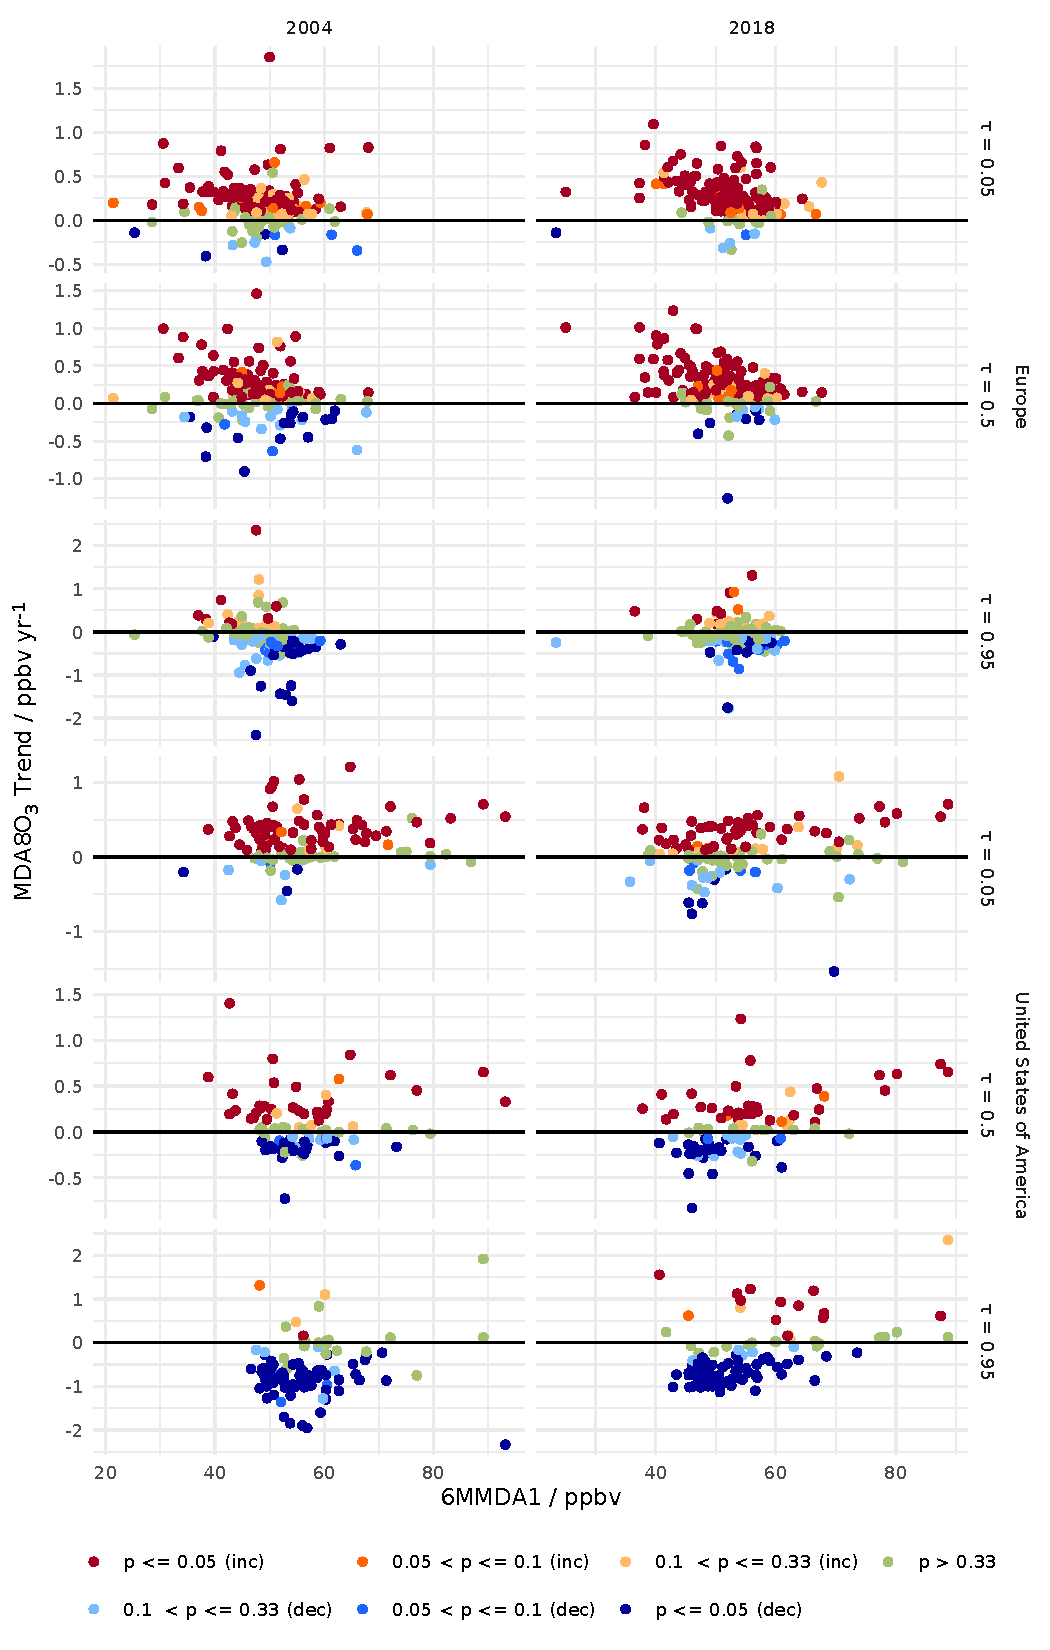
\includegraphics[height=0.75\textheight]{figures/si_figures/fS21_mda8_sig_mda8_6mmda1.pdf}
\caption{}
\label{si_fig:mda8_sig_mda8_6mmda1}
\end{figure}
\clearpage

\begin{figure}[p]
\centering
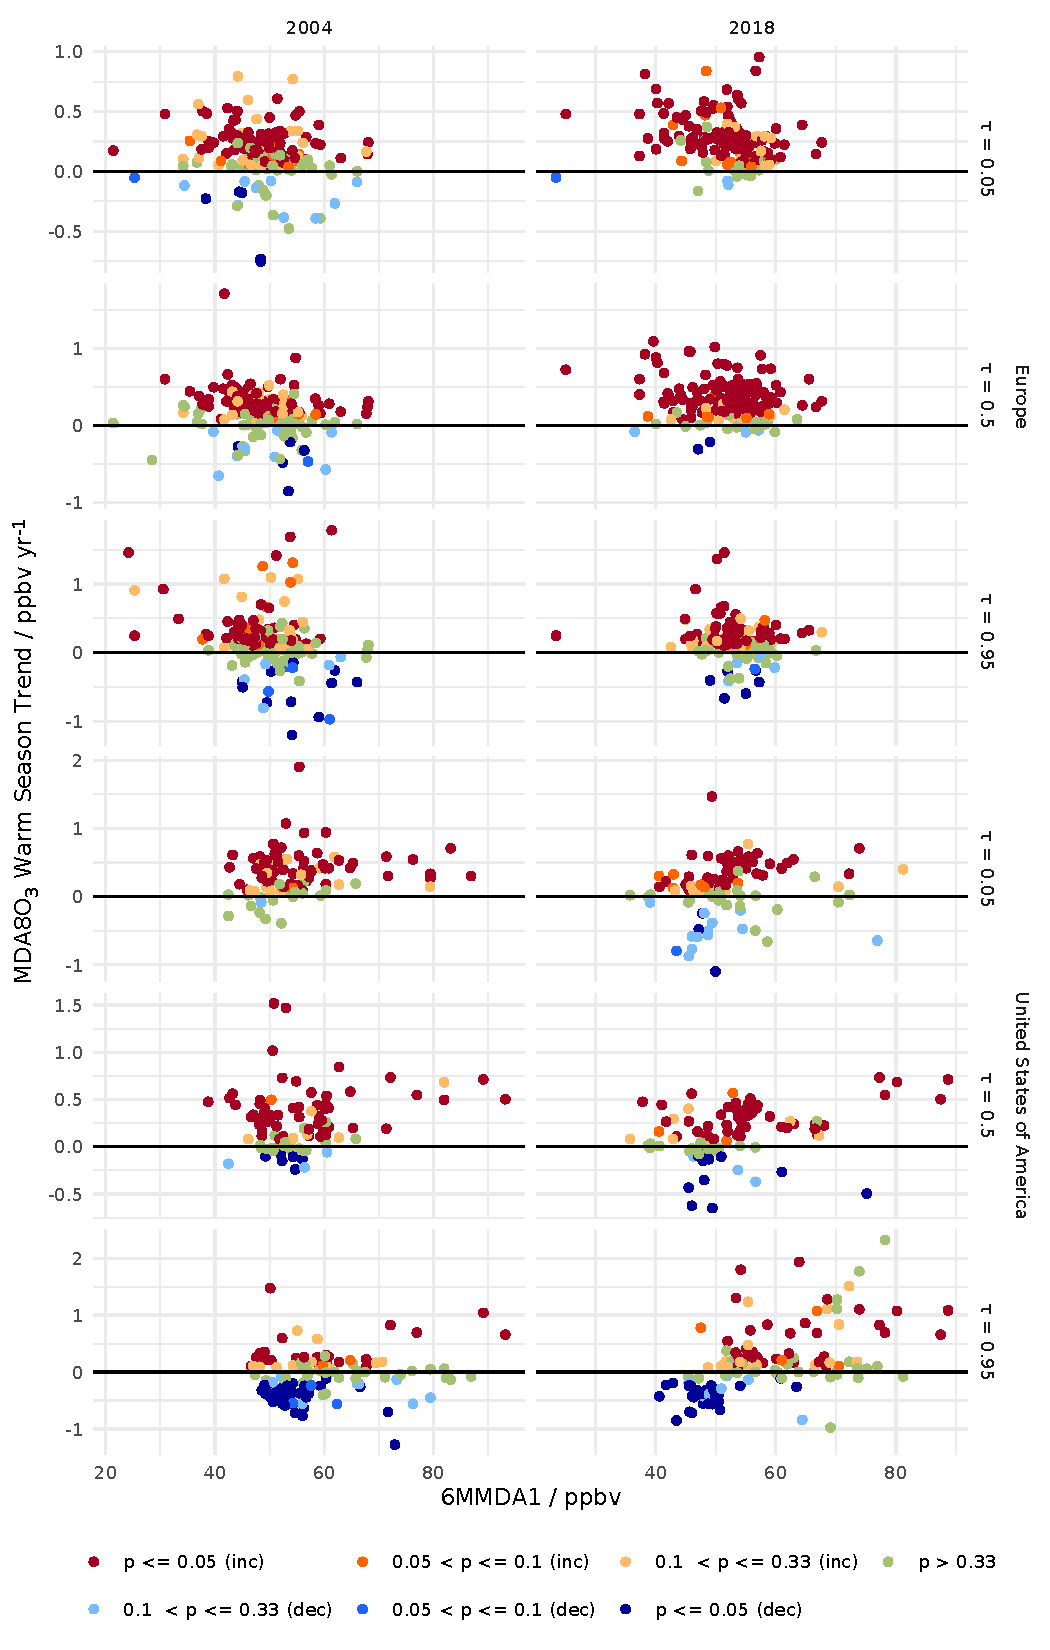
\includegraphics[height=0.75\textheight]{figures/si_figures/fS22_mda8_warm_sig_mda8_6mmda1.pdf}
\caption{}
\label{si_fig:mda8_warm_sig_mda8_6mmda1}
\end{figure}
\clearpage

\begin{figure}[p]
\centering
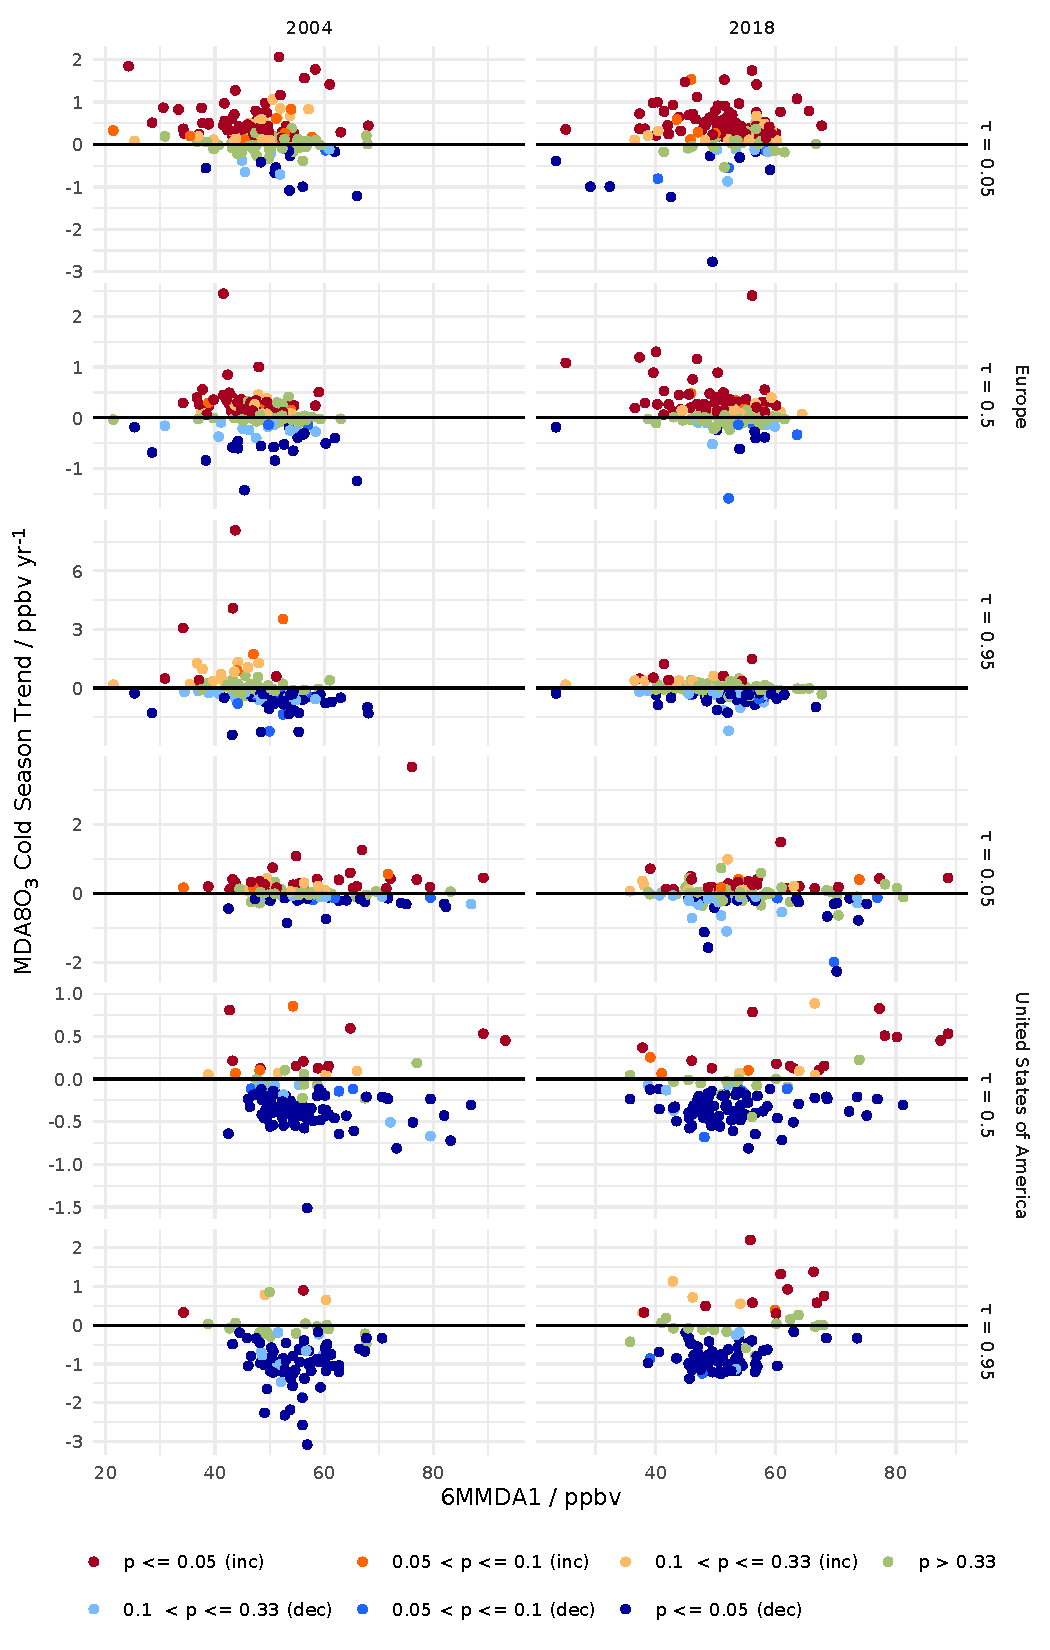
\includegraphics[height=0.75\textheight]{figures/si_figures/fS23_mda8_cold_sig_mda8_6mmda1.pdf}
\caption{}
\label{si_fig:mda8_cold_sig_mda8_6mmda1}
\end{figure}
\clearpage


%%%%%% tables %%%%%%


\end{document}

